\documentclass[12pt,a4paper]{article}
\usepackage[a4paper,top=2.55cm,bottom=2.55cm,left=2.55cm,right=2.55cm]{geometry}
\usepackage{fontspec}
\usepackage{xeCJK}
\usepackage{amsmath,amssymb}
\usepackage{xcolor}
\usepackage{booktabs}
\usepackage{tabularx}
\usepackage{colortbl}
\usepackage{graphicx}
\usepackage[most]{tcolorbox}
\usepackage{fancyhdr}
\usepackage{titlesec}
\usepackage{titletoc}
\usepackage{needspace}
\usepackage{array}
\usepackage{enumitem}
\usepackage[colorlinks=true,urlcolor=Primary,linkcolor=Ink,citecolor=Primary]{hyperref}

% 字体配置：优先使用 macOS 原生华文宋体常规体（FontIndex=6）与黑体，非 macOS 环境自动回退至 TeX Live 内置 Fandol / TeX Gyre 字体集
\IfFileExists{/System/Library/Fonts/Supplemental/Songti.ttc}{
  \setmainfont[
    Path=/System/Library/Fonts/Supplemental/,
    BoldFont=Times New Roman Bold.ttf,
    ItalicFont=Times New Roman Italic.ttf,
    BoldItalicFont=Times New Roman Bold Italic.ttf
  ]{Times New Roman.ttf}
  \setsansfont[
    Path=/System/Library/Fonts/Supplemental/,
    BoldFont=Arial Bold.ttf,
    ItalicFont=Arial Italic.ttf
  ]{Arial.ttf}
  \setCJKmainfont[
    Path=/System/Library/Fonts/Supplemental/,
    FontIndex=6,
    BoldFont=Songti.ttc,
    BoldFeatures={FontIndex=1}
  ]{Songti.ttc}
  \setCJKsansfont[
    Path=/System/Library/Fonts/,
    FontIndex=1,
    AutoFakeBold=1.5
  ]{STHeiti Medium.ttc}
}{
  \setmainfont{TeX Gyre Termes}
  \setsansfont{TeX Gyre Heros}
  \setCJKmainfont[BoldFont=FandolSong-Bold.otf]{FandolSong-Regular.otf}
  \setCJKsansfont[BoldFont=FandolHei-Bold.otf]{FandolHei-Regular.otf}
}

% 机构深酒红色板（Option A Burgundy）
\definecolor{Primary}{HTML}{8B1E24}
\definecolor{Secondary}{HTML}{9A7B4F}
\definecolor{Tertiary}{HTML}{3B6E5C}
\definecolor{BoxBg}{HTML}{FAF6F5}
\definecolor{KpiBg}{HTML}{F8F6F3}
\definecolor{TblHdr}{HTML}{F6F3F0}
\definecolor{RuleMuted}{HTML}{D8D2CA}
\definecolor{Ink}{HTML}{1E1E1E}
\definecolor{SubInk}{HTML}{4A4A4A}
\definecolor{GrayNote}{HTML}{666666}

\newcommand{\sqbullet}{\textcolor{Primary}{\rule[0.12em]{0.38em}{0.38em}}\hspace{0.38em}}

% 正文单套行距设置：12pt 字号配 18pt 基线距（精确 1.5 倍行距，不叠加 setspace 倍率）
\renewcommand{\normalsize}{\fontsize{12pt}{18pt}\selectfont}
\normalsize

% 页眉页脚（第2页起启用）
\setlength{\headheight}{14pt}
\pagestyle{fancy}
\fancyhf{}
\renewcommand{\headrulewidth}{0.4pt}
\renewcommand{\footrulewidth}{0.4pt}
\renewcommand{\headrule}{\hbox to\headwidth{\color{RuleMuted}\leaders\hrule height \headrulewidth\hfill}}
\renewcommand{\footrule}{\hbox to\headwidth{\color{RuleMuted}\leaders\hrule height \footrulewidth\hfill}}
\fancyhead[L]{\fontsize{9}{11}\selectfont\textcolor{SubInk}{列祖列宗量化 \textbar\ 金融工程与量化策略研究}}
\fancyhead[R]{\fontsize{9}{11}\selectfont\textcolor{SubInk}{沪深300价值低波多因子策略研究与私募产品化方案（M4）}}
\fancyfoot[L]{\fontsize{8.5}{10}\selectfont\textcolor{GrayNote}{《量化交易技术理论与实践》课程研究报告 \textbar\ 历史回测与模拟表现不构成投资建议}}
\fancyfoot[R]{\fontsize{9}{11}\selectfont\textcolor{SubInk}{第 \thepage\ 页}}

% 国内券商研报短标题层级样式（一、 / 1.1 / （1），关闭自动数字前缀使目录与书签单一干净）
\setcounter{secnumdepth}{0}
\setcounter{tocdepth}{2}
\titleformat{\section}{\sffamily\bfseries\fontsize{14pt}{19pt}\selectfont\color{Primary}}{}{0em}{}[\vspace{2pt}{\color{Primary}\titlerule[0.8pt]}]
\titlespacing*{\section}{0pt}{11pt}{6pt}

\titleformat{\subsection}{\sffamily\bfseries\fontsize{12.5pt}{17.5pt}\selectfont\color{Ink}}{}{0em}{}
\titlespacing*{\subsection}{0pt}{8.5pt}{3.5pt}

% 防止一级与二级标题孤立悬挂在页底
\let\origsection\section
\renewcommand{\section}[1]{\needspace{6.5\baselineskip}\origsection{#1}}
\let\origsubsection\subsection
\renewcommand{\subsection}[1]{\needspace{4\baselineskip}\origsubsection{#1}}

% 目录引导格式
\titlecontents{section}[0em]{\vspace{4pt}\sffamily\bfseries\fontsize{11pt}{15.5pt}\selectfont\color{Ink}}{}{}{\titlerule*[0.5pc]{.}\contentspage}
\titlecontents{subsection}[1.8em]{\fontsize{10.5pt}{14.8pt}\selectfont\color{SubInk}}{}{}{\titlerule*[0.5pc]{.}\contentspage}

\setlength{\parindent}{2em}
\setlength{\parskip}{2pt}
\widowpenalty=10000
\clubpenalty=10000
\emergencystretch=1.5em

% 统一图表容器宏（左对齐粗体题注 + 内容 + 左对齐紧凑资料来源与注释）
\newcommand{\exhibitcap}[1]{{\sffamily\bfseries\fontsize{9.6pt}{12.5pt}\selectfont\textcolor{Primary}{#1}}\\[2pt]}
\newcommand{\exhibitnote}[1]{{\fontsize{7.5pt}{10pt}\selectfont\color{GrayNote}#1\par}}

\begin{document}
\color{Ink}

% =========================================================================
% 第 1 页：券商金工深度研报式首页（严格 2.55cm 页边距，单页容纳，支持黑白打印）
% =========================================================================
\thispagestyle{empty}
{\setlength{\parindent}{0pt}\setlength{\parskip}{0pt}

% 1. 机构眉题（Masthead）
\begin{tabularx}{\textwidth}{@{}X r@{}}
  {\sffamily\bfseries\fontsize{12}{13.5}\selectfont\textcolor{Primary}{列祖列宗量化}\hspace{0.45em}\textcolor{RuleMuted}{|}\hspace{0.45em}\fontsize{9.2}{11}\selectfont\textcolor{SubInk}{金融工程与量化策略研究}} &
  {\sffamily\fontsize{8.6}{10.5}\selectfont\textcolor{Primary}{\bfseries 证券研究报告 · 深度专题}\hspace{0.5em}\textcolor{SubInk}{2026年12月}}
\end{tabularx}
\vspace{1.5pt}
{\color{Primary}\rule{\textwidth}{1.5pt}}\\[-8.5pt]
{\color{RuleMuted}\rule{\textwidth}{0.4pt}}

\vspace{4pt}

% 2. 主标题与明确口径副标题
{\sffamily\bfseries\fontsize{15}{19}\selectfont\textcolor{Ink}{沪深300价值低波多因子策略研究与私募产品化方案}}\\[2.5pt]
{\fontsize{7.45}{10}\selectfont\textcolor{SubInk}{\textbf{策略名称：}沪深300价值低波精选（M4）\hspace{0.45em}\textbf{角色定位：}私募证券投资基金量化投研团队\hspace{0.45em}\textbf{回测区间：}2023-01-09 至 2026-10-30（921交易日）}}

\vspace{4pt}

% 3. 五格核心指标带（第5格仅展示单次单边换手，彻底消除横向溢出）
\begin{tcolorbox}[
  enhanced,
  colback=KpiBg,
  colframe=RuleMuted,
  boxrule=0.4pt,
  borderline north={1.3pt}{0pt}{Primary},
  arc=0pt,
  left=2.5pt, right=2.5pt, top=3pt, bottom=3pt
]
\begin{tabularx}{\textwidth}{@{}*{5}{>{\centering\arraybackslash}X}@{}}
  \begin{tabular}[t]{@{}c@{}}
    {\fontsize{7.1}{8.8}\selectfont\textcolor{SubInk}{全期累计净收益}}\\[1pt]
    {\sffamily\bfseries\fontsize{11.5}{13}\selectfont\textcolor{Primary}{+56.58\%}}\\[0.5pt]
    {\fontsize{6.4}{7.8}\selectfont\textcolor{GrayNote}{含交易费·未扣产品费}}
  \end{tabular}
  &
  \begin{tabular}[t]{@{}c@{}}
    {\fontsize{7.1}{8.8}\selectfont\textcolor{SubInk}{相对价格指数累计差}}\\[1pt]
    {\sffamily\bfseries\fontsize{11.5}{13}\selectfont\textcolor{Ink}{+56.90 pct}}\\[0.5pt]
    {\fontsize{6.4}{7.8}\selectfont\textcolor{GrayNote}{沪深300价格指数 -0.33\%}}
  \end{tabular}
  &
  \begin{tabular}[t]{@{}c@{}}
    {\fontsize{7.1}{8.8}\selectfont\textcolor{SubInk}{几何年化 / 算术夏普}}\\[1pt]
    {\sffamily\bfseries\fontsize{11.5}{13}\selectfont\textcolor{Ink}{+13.05\% / 0.91}}\\[0.5pt]
    {\fontsize{6.4}{7.8}\selectfont\textcolor{GrayNote}{日频 $r_f=0$，IR 0.87}}
  \end{tabular}
  &
  \begin{tabular}[t]{@{}c@{}}
    {\fontsize{7.1}{8.8}\selectfont\textcolor{SubInk}{全期最大回撤}}\\[1pt]
    {\sffamily\bfseries\fontsize{11.5}{13}\selectfont\textcolor{Tertiary}{-15.88\%}}\\[0.5pt]
    {\fontsize{6.4}{7.8}\selectfont\textcolor{GrayNote}{同期价格指数 -24.80\%}}
  \end{tabular}
  &
  \begin{tabular}[t]{@{}c@{}}
    {\fontsize{7.1}{8.8}\selectfont\textcolor{SubInk}{单次单边换手}}\\[1pt]
    {\sffamily\bfseries\fontsize{11.5}{13}\selectfont\textcolor{Secondary}{2.74\%}}\\[0.5pt]
    {\fontsize{6.4}{7.8}\selectfont\textcolor{GrayNote}{5交易日调仓·前75缓冲}}
  \end{tabular}
\end{tabularx}
\end{tcolorbox}

\vspace{3pt}

% 4. 核心投资要点（Executive Summary）
{\sffamily\bfseries\fontsize{9.5}{12}\selectfont\textcolor{Primary}{核心投资要点（Executive Summary）}}
\vspace{1.5pt}

\begin{tcolorbox}[
  enhanced,
  colback=BoxBg,
  colframe=BoxBg,
  borderline west={2.3pt}{0pt}{Primary},
  arc=0pt,
  left=7pt, right=6.5pt, top=4pt, bottom=4pt
]
\fontsize{8.3}{11.7}\selectfont
\sqbullet\textbf{低换手价值低波框架压降交易摩擦损耗：}在 2023-01-09 至 2026-10-30 实盘约束回测（计双边万3佣金、千1滑点及固定卖出千1印花税，未扣产品费）中，高换手量价对照（M0b，每5交易日调仓）单次单边换手达 51.70\%，毛收益 +28.54\% 扣费后转为 -8.88\%。M4 以账面市值比（BP）、盈利收益率（EP）与经行业市值中性化的60日低波、20日低换手四因子等权打分，配合 Top 50 等权与前75名保留缓冲带，将单次单边换手压至 2.74\%，累计净收益 +56.58\%（几何年化 +13.05\%；组合后复权含现金分红，对比基准沪深300价格指数不含分红）。\\[2.5pt]
\sqbullet\textbf{双股票池回测权衡与横截面归因分解：}沪深300同池内五因子 M5 的收益、夏普与回撤优于 M4，且 M4 在历史留后区间收益（+12.21\%）低于基准模型 M1（+14.07\%）；但同规格用于中证500后，M4 在全期净收益（+57.73\%）、夏普（0.816）与最大回撤（-16.46\%）三项指标上均优于 M5 并居全池首位。综合跨池一致性与减少派生因子的简洁性选定 M4。在该滞后持仓7因子横截面回归设定下，沪深300组合中低波与低换手合计贡献 +2.49 个百分点/年。\\[2.5pt]
\sqbullet\textbf{容量执行情景、历史模拟费后表现与模拟跟踪：}按5\%日均成交参与率上限测算，5亿元规模下单日调仓与假设3日均分拆单分别有 38/184 期与 4/184 期超限（主回测采用次日开盘集中撮合，多日拆单属独立执行情景）。在机构C档费率（0.60\%管理费+0.15\%托管费，相对沪深300价格指数超额收益按年度高水位计提15\%）下，扣除产品费后的历史模拟年化收益为 +10.39\%。雪球公开组合 ZH3689205 归档运行记录披露至 2026-11-23，与50股主回测及30股历史映射分列呈现。\par
\end{tcolorbox}

\vspace{3pt}

% 5. 图表 1：首页全宽主净值走势图
{\sffamily\bfseries\fontsize{8.4}{10.5}\selectfont\textcolor{Primary}{图表 1：沪深300核心消融组合与价格指数累计净值走势（2023-01-09 至 2026-10-30）}}\\[1.5pt]
{\color{Primary}\rule{\textwidth}{0.8pt}}\\[1pt]
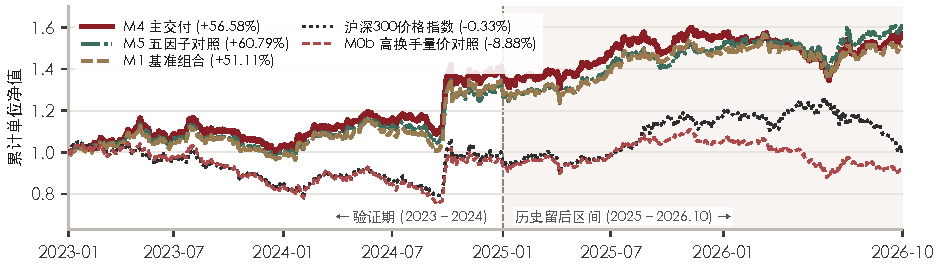
\includegraphics[width=\textwidth]{../figures/report_tex/fig01_cover_nav.pdf}\\[-3pt]
{\color{Primary}\rule{\textwidth}{0.6pt}}\\[1.5pt]
{\fontsize{6.8}{8.6}\selectfont\color{GrayNote}资料来源：个股后复权日行情源自 Tushare 官方接口，沪深300价格指数（000300.SH）源自随包历史行情表，列祖列宗量化投研部测算。注：组合净值已扣双边万3佣金、千1滑点与固定卖出千1印花税（未扣产品费），含分红再投资；价格指数不含分红，首日按2023-01-09开盘对齐为1.00；2025-01-02至2026-10-30为已参与方案讨论的历史留后区间。\par}

\vfill

% 6. 团队成员信息、开源仓库与雪球公开链接（各独立成行）
{\color{Primary}\rule{\textwidth}{0.8pt}}
\vspace{2pt}
{\renewcommand{\arraystretch}{1.14}\fontsize{7.55}{9.7}\selectfont
\begin{tabularx}{\textwidth}{@{}l >{\raggedright\arraybackslash}X@{}}
  \textbf{\sffamily\textcolor{Primary}{课程与指导教师：}} &
  《量化交易技术理论与实践》期末书面技术报告 \hspace{1.2em} \textbf{指导教师：}肖亮海 \\
  \textbf{\sffamily\textcolor{Primary}{研究团队与分工：}} &
  李钰鹏（2024104286，双池时点数据治理） \textperiodcentered\ 刘宇睿（2024101054，因子重筛与消融建模） \textperiodcentered\ 张沐（2024101056，无前视回测与归因） \textperiodcentered\ 张恒瑞（2024101062，容量费率测算与总报告整合） \\
  \textbf{\sffamily\textcolor{Primary}{代码开源仓库：}} &
  \url{https://github.com/z2823253773-p/csi300-quant-strategy} \\
  \textbf{\sffamily\textcolor{Primary}{雪球公开模拟盘：}} &
  \url{https://www.xueqiu.com/P/ZH3689205}（组合名称：沪深300价值精选，公开组合代号：ZH3689205）
\end{tabularx}\par}
\vspace{1.5pt}
{\color{RuleMuted}\rule{\textwidth}{0.4pt}}\\[1pt]
{\fontsize{6.7}{8.2}\selectfont\color{GrayNote}声明：本报告由“列祖列宗量化”课程团队独立完成，仅供课程考核与模拟投委会评审使用，历史回测与模拟表现不构成投资建议。\hfill 第 1 页\par}
}

\newpage

% =========================================================================
% 第 2 页：目录与核心图表索引
% =========================================================================
{\setlength{\parindent}{0pt}
{\sffamily\bfseries\fontsize{15pt}{20pt}\selectfont\textcolor{Primary}{目\hspace{1em}录}}\\[3pt]
{\color{Primary}\rule{\textwidth}{1.0pt}}
\vspace{4pt}
{\makeatletter\@starttoc{toc}\makeatother}
}

\vspace{10pt}
{\setlength{\parindent}{0pt}
{\sffamily\bfseries\fontsize{11pt}{15pt}\selectfont\textcolor{Primary}{核心图表与实证模块导览}}\\[2pt]
{\color{RuleMuted}\rule{\textwidth}{0.5pt}}\\[4pt]
{\fontsize{8.2pt}{11.5pt}\selectfont\color{SubInk}
\begin{tabularx}{\textwidth}{@{}l X@{}}
  \textbf{图表 1--2} & 首页沪深300核心消融净值走势、四阶段量化投研与产品化流水线架构图 \\
  \textbf{图表 3--5} & 双股票池底层面板规模与防前视时效参数、候选因子数学定义、M0a--M5 控制变量消融矩阵 \\
  \textbf{图表 6--8} & 双股票池训练期 Alpha101 全量重筛入选结果、分阶段 5 日 Rank IC 均值对照表与柱状图 \\
  \textbf{图表 9--12} & 双股票池回测绩效与选型主表、中证500净值与双池夏普对比、Alpha015 低覆盖约束传导诊断 \\
  \textbf{图表 13--17} & 滞后实际持仓 7 因子 Fama-MacBeth 归因表与分解图、申万一级行业集中度表与水下回撤曲线 \\
  \textbf{图表 18--22} & 私募产品要素与客户分层表、四档高水位费后模拟表与净值图、双池流动性与容量情景压测 \\
  \textbf{图表 23--27} & 雪球 30 股历史映射与实盘归档分列表、近 8 期调仓明细、平台截图凭证及可复现工程字段映射表 \\
\end{tabularx}\par}
}

\newpage

% =========================================================================
% 一、研究背景与策略投资框架
% =========================================================================
\section{一、研究背景与策略投资框架}

\subsection{1.1 大盘宽基被动配置痛点与量化多因子定位}

在 A 股机构化配置体系中，沪深300指数覆盖两市核心龙头资产，具备充沛的单票流动性与清晰的治理结构，长期承担机构底仓基准职能。然而，单纯持有市值加权宽基指数在回测区间（2023-01-09 至 2026-10-30，共 921 个交易日）内面临两项现实约束：一是市值加权机制在风格周期顶部容易对高估值板块赋予较高权重，期间沪深300价格指数累计变动 -0.33\%，最大回撤达 -24.80\%；二是若试图直接移植高频短周期量价公式进行周度选股，A 股特有的卖出印花税、交易佣金与盘口冲击成本将迅速侵蚀选股毛收益。

围绕私募证券投资基金量化投研团队的角色定位，本研究旨在回答三个层面的工程与投资问题：第一，在严格消除幸存者偏差与时点前视偏差的前提下，经典短窗公式化量价因子与中低频基本面、低风险因子在大盘股与中盘股中各自表现如何；第二，当多因子研究涉及共同选股池交集、因子衍生比率与周度调仓摩擦时，如何通过控制变量实验识别收益来源与工程隐患；第三，在计入产品层管理费、托管费、年度高水位业绩报酬以及成交参与率上限后，策略在何种资金规模与执行假设下具备实际可落地性。

\subsection{1.2 价值低波四因子等权与排名缓冲带设计}

针对大盘蓝筹股票池机构定价效率较高、高频反转信号半衰期较短的特征，本研究构建的主交付策略“沪深300价值低波精选（M4）”采用纯多头（Long-Only）、等权合成与排名缓冲降耗的投资框架，由三项核心机制组成：

（1）\textbf{价值双锚刻画安全边际与真实盈利回报。}组合以账面市值比（$\text{BP} = 1/\text{PB}$）衡量净资产折价保护，同时引入盈利收益率（$\text{EP} = 1/\text{PE}$，当期亏损标的保留为空值而不做零值填补）过滤账面低估但持续亏损的标的。两项价值因子不做行业中性化处理，用保留跨行业估值比价的方式捕捉大盘低估值板块的配置收益，同时将由此产生的金融板块暴露纳入第四章专项风险审计。

（2）\textbf{行业市值中性化低风险双因子提供防御互补。}受个人投资者高波动偏好与杠杆约束影响（Frazzini \& Pedersen, 2014），A 股高波动、高换手标的在截面上长期呈现负向风险调整后溢价。本研究引入经申万一级行业与对数流通市值代理横截面正交化后的60日低波动因子与20日低换手因子，在不额外叠加银行股行业权重的前提下筛选筹码结构稳定、特质波动温和的成分股。

（3）\textbf{四因子直接等权与前75名保留缓冲带控制换手。}为降低样本内参数寻优带来的过拟合风险，组合对四项截面标准化因子赋予固定等权重（各 25\%），每 5 个交易日生成一次信号，目标持有 50 只等权标的（单只目标权重 2.00\%）。调仓引入“前 75 名保留缓冲带”规则：上期目标持仓若当期综合得分仍居共同选股池前 75 名则予以保留，空缺席位再由未持仓高分标的按序递补。该机制将沪深300 M4 常规调仓的平均单次单边换手压降至 2.74\%。

\vspace{4pt}
\noindent\begin{minipage}{\textwidth}
\setlength{\parindent}{0pt}
\exhibitcap{图表 2：双股票池多因子研究、无前视回测与私募产品化四阶段架构图}
{\color{Primary}\rule{\textwidth}{0.8pt}}\\[2pt]
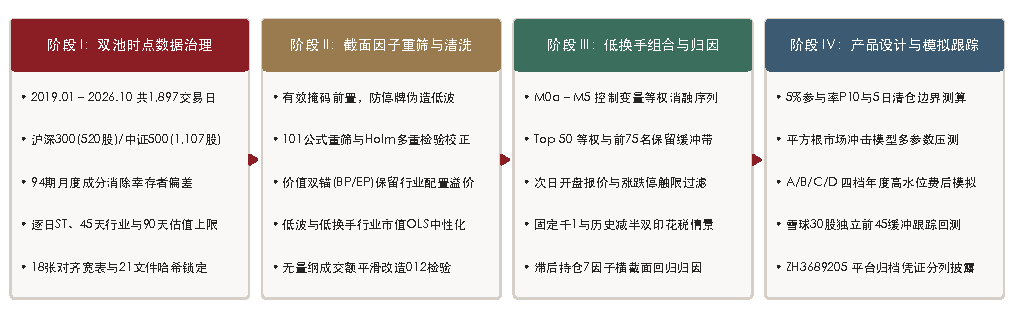
\includegraphics[width=\textwidth]{../figures/report_tex/fig02_framework_flow.pdf}\\[-2pt]
{\color{Primary}\rule{\textwidth}{0.6pt}}\\[2pt]
\exhibitnote{资料来源：列祖列宗量化投研部绘制。注：四个阶段之间通过只读标准化数据表与文件哈希校验衔接，任一阶段不回调修改上游原始输入。}
\end{minipage}
\vspace{5pt}

\subsection{1.3 投研流水线协同与跨模块校验机制}

如上图所示，全流程按机构投研分工拆解为数据工程、因子与消融信号、无前视账户回测与归因、产品化设计与模拟跟踪四个独立模块。上游数据层交付经 21 项文件 SHA-256 指纹锁定的双池标准面板；信号层通过前缀截断因果性测试与权重和恒等校验；回测层在 3 组实验池、21 个策略账户与 3 类费率假设（共 63 组净值序列）上实现逐日资产恒等式零残差闭合，并经两套独立代码交叉复算核对；产品与报告层通过统一路径解析器自动汇总各阶段产出表，并与雪球平台本地归档核验记录做分口径披露。

% =========================================================================
% 二、数据治理与多因子体系构建
% =========================================================================
\section{二、数据治理与多因子体系构建}

\subsection{2.1 双股票池动态成分构建与时点防前视规则}

为同时评估策略在沪深300大盘池的主体表现及在中证500中盘池的跨池适用性，研究底层统一覆盖 2019-01-02 至 2026-10-30 共 1,897 个交易日（其中 2019 年至 2022 年为因子筛选与特征观察的训练期，2023 年 1 月起进入组合账户回测期）。数据来源按字段严格区分：个股日线行情（开盘、最高、最低、收盘、成交量、成交额）、估值指标（市盈率 TTM、市净率 MRQ）、日换手率、复权因子及历史风险警示（ST）变更记录拉取自 Tushare 官方接口；94 期月度指数成分股历史快照、申万一级行业历史变更记录与沪深300（000300.SH）、中证500（000905.SH）价格指数日行情采用随包核对的历史种子文件。

在时点数据清洗与单位标准化环节，工程管道执行四项硬性规范：第一，\textbf{动态成分映射消除幸存者偏差}，沪深300与中证500全样本分别纳入历史进出成分股 520 只与 1107 只，对证券代码变更事件（如中航电测由 300114.SZ 变更为 302132.SZ）按同一证券连续拼接，对停牌或无报价日严格保留空报价状态而不伪造可成交价格；第二，\textbf{行业与估值快照时效上限}，申万一级行业历史映射限定最长向前沿用 45 天，超出时效或早期缺失样本单独归入“未分类”哑变量组（沪深300与中证500全样本未分类占比分别为 19.47\% 与 15.63\%），估值指标限定最长向前沿用 90 天且非正值直接置空；第三，\textbf{逐日风险警示状态还原}，按交易日逐日标记 ST 状态，避免将后续年份才被实施风险警示的个股提前在正常交易年份剔除或错误套用 4.5\% 涨跌停阈值；第四，\textbf{量价单位截面核验}，成交量统一换算为股、成交额统一换算为人民币元，在 2026-10-30 截面上实测成交额与“成交量 $\times$ 未复权收盘价”比值的中位数为 1.0052，确认底层流动性测算不存在千倍或百倍单位错位。

\vspace{4pt}
\noindent\begin{minipage}{\textwidth}
\setlength{\parindent}{0pt}\setlength{\tabcolsep}{4.5pt}
\exhibitcap{图表 3：沪深300与中证500双股票池底层面板规模与时效治理参数表}
\fontsize{8.0pt}{11pt}\selectfont
\begin{tabularx}{\textwidth}{@{}X r r l@{}}
  \arrayrulecolor{Primary}\toprule[1.0pt]
  \rowcolor{TblHdr}
  \textbf{\sffamily 数据治理维度与时点约束指标} & \textbf{\sffamily 沪深300股票池} & \textbf{\sffamily 中证500股票池} & \textbf{\sffamily 防前视与数据质量控制说明} \\
  \midrule[0.5pt]
  样本时间跨度（训练期 + 回测期） & 1,897 交易日 & 1,897 交易日 & 2019-01-02 至 2026-10-30 \\
  历史动态进出成分股总数 & 520 只 & 1107 只 & 基于 94 期月度历史成分快照逐日映射 \\
  日频长面板总观测行数 & 940,701 行 & 1,943,001 行 & 跨池重复标的底层仅拉取一次，口径统一 \\
  正常可交易有效观测行数 & 568,037 行 & 946,149 行 & 正常交易、非停牌且开高低收量齐全且量 $>0$ \\
  估值指标向前沿用上限 & 90 自然日 & 90 自然日 & 亏损或净资产非正直接留空，不作零值填充 \\
  申万一级行业快照时效上限 & 45 自然日 & 45 自然日 & 剔除事后行业回填，超期归入独立未分类组 \\
  行业未分类样本占比 & 19.47\% & 15.63\% & 横截面回归时单独设立未分类行业哑变量 \\
  流通市值代理有效覆盖率 & 100.0\% & 100.0\% & 由日成交额除以换手率构造对数流通市值代理 \\
  对齐宽表与输入哈希锁定文件数 & 18 张 / 21 项 & 18 张 / 21 项 & 宽表行列严格对齐，SHA-256 指纹自动核验 \\
  \arrayrulecolor{Primary}\bottomrule[1.0pt]
\end{tabularx}\\[3pt]
\exhibitnote{资料来源：Tushare 官方接口与随包历史成分及申万行业种子表，列祖列宗量化投研部整理。}
\end{minipage}
\vspace{5pt}

\subsection{2.2 截面清洗公理与候选因子数学定义}

在日频多因子计算中，若先对停牌期间的价格序列做向前填充，再计算滚动收益率标准差或均值，长期停牌股将因连续零收益被错误识别为“极低波动、极低换手”标的。为此，本研究确立\textbf{有效观测掩码前置公理}：记股票 $i$ 在交易日 $t$ 的原始有效交易指示变量为 $V_{i,t} \in \{0, 1\}$（当且仅当当日正常交易、非停牌、开高低收报价均有效且成交量严格大于零时取 1），一切滚动窗口、一阶差分与指数平滑算子均在经 $V_{i,t}$ 置空后的序列上执行。

设股票 $i$ 在 $t$ 日的后复权收盘价收益率（仅在相邻有效交易观测间计算）为 $r_{i,t}$，日成交额（元）为 $\text{Amt}_{i,t}$，日换手率（百分比数值）为 $\text{Turn}_{i,t}$。本研究涉及的核心基本面、低风险与衍生/改造量价因子定义如下：

第一，\textbf{价值双锚与对数流通市值代理因子}：
\begin{equation}
\text{BP}_{i,t} = \frac{1}{\text{PB\_MRQ}_{i,t}}, \qquad
\text{EP}_{i,t} = \begin{cases} 1 / \text{PE\_TTM}_{i,t}, & \text{PE\_TTM}_{i,t} > 0 \\ \text{NaN}, & \text{PE\_TTM}_{i,t} \le 0 \end{cases}
\end{equation}
\begin{equation}
\text{LnFloatMV}_{i,t} = \ln\!\left(\frac{\text{Amt}_{i,t}}{\text{Turn}_{i,t} / 100}\right), \qquad \text{Small}_{i,t} = -\text{LnFloatMV}_{i,t}
\end{equation}

第二，\textbf{60日低波动与20日低换手防御因子}（分别要求最近 60 个交易日内有效观测不少于 40 天、最近 20 个交易日内严格正换手观测不少于 15 天）：
\begin{equation}
\text{LowVol60}_{i,t} = -\sqrt{\frac{1}{|W_{60}(i,t)| - 1} \sum_{\tau \in W_{60}(i,t)} \left(r_{i,\tau} - \bar{r}_{i,60}\right)^2}
\end{equation}
\begin{equation}
\text{LowTurn20}_{i,t} = -\ln\!\left(\frac{1}{|W_{20}(i,t)|} \sum_{\tau \in W_{20}(i,t)} \text{Turn}_{i,\tau}\right)
\end{equation}

第三，\textbf{隐含账面盈利率比率代理与无量纲成交额平滑改造动量因子}。在五因子对照模型 M5 中，为考察在不接入外部季度财报库时能否补充盈利效率信息，构造由盈利收益率与账面市值比直接相除的比率代理：
\begin{equation}
\text{EB\_Proxy}_{i,t} = \frac{\text{EP}_{i,t}}{\text{BP}_{i,t}}, \qquad (\text{要求 } \text{BP}_{i,t} > 0 \text{ 且 } \text{EP}_{i,t} \text{ 非空})
\end{equation}
在量价因子改造方面，Kakushadze（2016）原始 Alpha012 公式为 $-\operatorname{sign}(\Delta \text{Volume}_{i,t}) \cdot \Delta \text{Close}_{i,t}$，因直接乘以未标准化绝对价差 $\Delta \text{Close}_{i,t}$，在名义股价相差百倍的成分股截面上存在明显的价格尺度偏差（价格缩放 0.1 倍至 10 倍测试下截面排序改变；在沪深300训练期，仅将绝对价差替换为相对收益率即可使 5 日平均 Rank IC 由 +0.0046 升至 +0.0096）。本研究进一步将成交量变化替换为成交额变化，并施加半衰期匹配的 10 日指数移动平均（要求至少 5 个有效观测且当日量价冲击有效），构造无量纲成交额平滑改造因子：
\begin{equation}
\text{New012}_{i,t} = \operatorname{EMA}_{10}\!\Big(-\operatorname{sign}\!\left(\text{Amt}_{i,t} - \text{Amt}_{i,t-1}\right) \cdot r_{i,t}\Big)
\end{equation}
需要明确界定的是，式（6）相对原始 Alpha012 同步改动了价格无量纲化、成交额替代成交量以及 10 日平滑三项设定，因此后续组合回测中观测到的绩效变化属于三项改动的联合效应，不能单独归因于其中某一项子改动。

在每个交易日 $t$ 的当日可交易成分股截面内，各原始因子 $f_{i,t}$ 依次经过两步或三步标准化处理：首先按中位数绝对偏差执行稳健去极值，将超出 $\operatorname{Med}(f_t) \pm 5 \times 1.4826 \times \operatorname{MAD}(f_t)$ 的极端值截断至边界（当离散度退化为零时回退采用四分位距 $\operatorname{IQR}/1.349$）；其次，除保留原始风格配置属性的 $\text{BP}$、$\text{EP}$ 与 $\text{Small}$ 外，其余低风险、量价与比率代理因子均对申万一级行业哑变量矩阵 $D_{i,t}$（含未分类组）及标准化对数流通市值代理做横截面普通最小二乘（OLS）回归取残差 $\varepsilon_{i,t}$：
\begin{equation}
\tilde{f}_{i,t} = \alpha_t + \beta_t \, z\!\left(\text{LnFloatMV}_{i,t}\right) + \sum_{k} \gamma_{k,t} D_{i,k,t} + \varepsilon_{i,t}, \qquad z_{i,t} = \frac{\varepsilon_{i,t} - \bar{\varepsilon}_t}{\sigma(\varepsilon_t)}
\end{equation}
最后统一标准化为截面均值 0、样本标准差 1 的无量纲得分 $z_{i,t}$。

\vspace{4pt}
\noindent\begin{minipage}{\textwidth}
\setlength{\parindent}{0pt}\setlength{\tabcolsep}{3.8pt}
\exhibitcap{图表 4：候选基本面、低风险与量价因子定义及截面预处理规范表}
\fontsize{7.8pt}{10.6pt}\selectfont
\begin{tabularx}{\textwidth}{@{}l l c X@{}}
  \arrayrulecolor{Primary}\toprule[1.0pt]
  \rowcolor{TblHdr}
  \textbf{\sffamily 因子名称} & \textbf{\sffamily 核心数学表达} & \textbf{\sffamily 行业市值中性化} & \textbf{\sffamily 金融学含义与数据处理边界} \\
  \midrule[0.5pt]
  账面市值比（BP） & $1 / \text{PB\_MRQ}_{i,t}$ & 否 & 表征净资产折价安全边际，保留低估值行业配置溢价 \\
  盈利收益率（EP） & $1 / \text{PE\_TTM}_{i,t}$（正值有效） & 否 & 剔除当期亏损标的，防范单纯低市净率的价值陷阱 \\
  小市值代理（Small） & $-\ln(\text{Amt}_{i,t} / (\text{Turn}_{i,t}/100))$ & 否 & 历史基准组成部分，平衡超大市值权重股集中度 \\
  60日低波动（LowVol60） & $-\operatorname{std}_{60}(r_{i,t})$（$\ge 40$有效日） & 是 & 剥离行业与规模效应后的低特质收益波动溢价 \\
  20日低换手（LowTurn20） & $-\ln(\overline{\text{Turn}}_{20})$（$\ge 15$有效日） & 是 & 规避短期交易拥挤与高换手博弈标的，自相关性高 \\
  隐含账面盈利率代理 & $\text{EP}_{i,t} / \text{BP}_{i,t}$（$\text{BP}>0$） & 是 & 由估值比率相除派生，不等同于按财报公告日对齐的会计 ROE \\
  成交额平滑改造012 & $\operatorname{EMA}_{10}(-\operatorname{sign}(\Delta\text{Amt}_t)\cdot r_t)$ & 是 & 消除名义股价量纲偏差并适配周度调仓持有周期 \\
  全量重筛 Alpha101 & Kakushadze（2016）附录公式 & 是 & 双股票池各自在训练期经 101 次检验 Holm 校正筛选前3席 \\
  \arrayrulecolor{Primary}\bottomrule[1.0pt]
\end{tabularx}\\[3pt]
\exhibitnote{资料来源：列祖列宗量化投研部整理。注：所有因子均严格遵循有效观测掩码前置公理，杜绝停牌前填伪造低波或低换手信号。}
\end{minipage}
\vspace{5pt}

\subsection{2.3 控制变量消融实验矩阵设定}

为避免同时变更选股池、打分公式、调仓周期与缓冲带导致绩效差异无法归因，本研究构建了从历史基线（M0a、M0b）到控制变量消融组（M1 至 M5）的八模型序列（见图表 5）。在共同池消融组（M1 至 M5）内部，所有模型统一采用每 5 个交易日调仓、目标持有前 50 只等权、上期目标持仓前 75 名保留缓冲带的组合构建规则，并在每个信号日共享同一共同有效股票集（得分并列时按证券代码升序稳定打破平局）。历史基线 M0a 与 M0b 则保留前期研究的无缓冲规则与原始基线入池口径，作为高换手成本损耗与规则演进的参照锚点。

\vspace{4pt}
\noindent\begin{minipage}{\textwidth}
\setlength{\parindent}{0pt}\setlength{\tabcolsep}{3.8pt}
\exhibitcap{图表 5：历史基线与共同池控制变量消融实验（M0a 至 M5）规格表}
\fontsize{7.8pt}{10.6pt}\selectfont
\begin{tabularx}{\textwidth}{@{}l l l X@{}}
  \arrayrulecolor{Primary}\toprule[1.0pt]
  \rowcolor{TblHdr}
  \textbf{\sffamily 模型代号} & \textbf{\sffamily 截面综合打分公式} & \textbf{\sffamily 持仓与缓冲机制} & \textbf{\sffamily 对照目的与拟检验的核心问题} \\
  \midrule[0.5pt]
  M0a（历史基线1） & $B = (z_{\text{BP}} + z_{\text{EP}} + z_{\text{Small}})/3$ & 5日，前50等权，无缓冲 & 保留早期三因子无缓冲基线口径作为参照起点 \\
  M0b（历史基线2） & $0.50 B + 0.25 z_{\text{A006}} + 0.25 z_{\text{A033}}$ & 5日，前50等权，无缓冲 & 展示50\%短窗量价权重在周度调仓下的交易摩擦损耗 \\
  M1（共同池基准） & $B = (z_{\text{BP}} + z_{\text{EP}} + z_{\text{Small}})/3$ & 5日，前50等权，前75缓冲 & 共同池控制变量基准（较M0a同步改变缓冲与入池口径） \\
  M2（纯价值底盘） & $V = Z\big((z_{\text{BP}} + z_{\text{EP}})/2\big)$ & 同 M1 & 剥离小市值代理，检验规模暴露在大盘与中盘池的差异 \\
  M3a（重筛Alpha） & $0.90 B + 0.10 \times \overline{z}_{\text{入选3项Alpha}}$ & 同 M1 & 检验经Holm校正入选的10\%量价因子能否增厚扣费净值 \\
  M3b（改造012） & $0.85 V + 0.15 z_{\text{New012}}$ & 同 M1 & 相对同底盘M2检验无量纲成交额平滑因子的跨池净效应 \\
  \textbf{\textcolor{Primary}{M4（主交付）}} & \textbf{\textcolor{Primary}{$(z_{\text{BP}} + z_{\text{EP}} + z_{\text{LowVol60}} + z_{\text{LowTurn20}})/4$}} & \textbf{同 M1} & \textbf{检验价值双锚叠加中性化低波低换手的跨池风险收益表现} \\
  M5（五因子对照） & $(z_{\text{BP}} + z_{\text{EP}} + z_{\text{LowVol60}} + z_{\text{LowTurn20}} + z_{\text{EB}})/5$ & 同 M1 & 相对M4检验增补EP/BP派生比率因子是否带来稳健增量 \\
  \arrayrulecolor{Primary}\bottomrule[1.0pt]
\end{tabularx}\\[3pt]
\exhibitnote{资料来源：列祖列宗量化投研部整理。注：$Z(\cdot)$ 表示对合成均值再做一次当日截面标准化，使 M3b 中纯价值底盘与改造动量因子处于同一标准差量纲。}
\end{minipage}
\vspace{4pt}

% =========================================================================
% 三、单因子检验、双股票池回测与 M4 选型
% =========================================================================
\section{三、单因子检验、双股票池回测与 M4 选型}

\subsection{3.1 Alpha101 全量重筛、比例化改进与单因子检验}

为克服主观挑选少数公式化量价因子的局限，研究在沪深300与中证500两个动态池上各自完成了 Kakushadze（2016）全部 101 个公式的本地化实现（其中两池均有 98 个公式在三阶段具备有效截面 Rank IC，第 7、96、97 号因严格完整窗口或截尾尺度退化为空）。筛选规则严格锁定在训练期（2019–2022）内执行：要求非行业市值代理变体、训练期有效交易日不少于 600 天、平均截面覆盖率不低于 60\%，且经 Newey-West（1987）异方差自相关稳健标准误计算的 $t$ 统计量通过 101 次多重检验 Holm（1979）序贯校正（$p_{\text{Holm}} \le 0.05$）；通过门槛的候选因子按训练期 5 日平均 Rank IC 绝对值降序排列，剔除与已入选因子截面秩相关绝对值 $\ge 0.70$ 的高度共线项后，每池至多保留前 3 席，因子符号完全由训练期决定。

\vspace{4pt}
\noindent\begin{minipage}{\textwidth}
\setlength{\parindent}{0pt}\setlength{\tabcolsep}{3.8pt}
\exhibitcap{图表 6：双股票池训练期 Alpha101 全量重筛入选因子三阶段 5 日 Rank IC 与覆盖率表}
\fontsize{7.8pt}{10.6pt}\selectfont
\begin{tabularx}{\textwidth}{@{}l X r r r r r r@{}}
  \arrayrulecolor{Primary}\toprule[1.0pt]
  \rowcolor{TblHdr}
  \textbf{\sffamily 股票池} & \textbf{\sffamily 入选因子} & \textbf{\sffamily 训练期 IC} & \textbf{\sffamily HAC-$t$} & \textbf{\sffamily Holm 校正 $p$} & \textbf{\sffamily 验证期 IC} & \textbf{\sffamily 历史留后 IC} & \textbf{\sffamily 三阶段覆盖率（训/验/后，\%）} \\
  \midrule[0.5pt]
    沪深300 & Alpha040 & +0.0218 & 4.43 & 0.0009 & +0.0200 & +0.0225 & 98.8 / 99.9 / 99.9 \\
    沪深300 & Alpha006 & +0.0199 & 4.31 & 0.0016 & +0.0011 & +0.0153 & 98.8 / 99.9 / 99.9 \\
    沪深300 & Alpha015 & +0.0162 & 4.44 & 0.0009 & +0.0083 & +0.0184 & 61.6 / 52.4 / 56.9 \\
    \arrayrulecolor{RuleMuted}\midrule[0.35pt]
    中证500 & Alpha040 & +0.0300 & 6.52 & 6.33e-09 & +0.0271 & +0.0228 & 98.8 / 99.9 / 99.9 \\
    中证500 & Alpha013 & +0.0253 & 7.91 & 2.56e-13 & +0.0161 & +0.0222 & 99.2 / 99.6 / 99.6 \\
    中证500 & Alpha044 & +0.0244 & 7.40 & 1.36e-11 & +0.0102 & +0.0264 & 99.1 / 99.5 / 99.5 \\
  \arrayrulecolor{Primary}\bottomrule[1.0pt]
\end{tabularx}\\[3pt]
\exhibitnote{资料来源：Tushare 后复权日线行情，列祖列宗量化投研部测算。注：训练期为 2019–2022 年，验证期为 2023–2024 年，历史留后区间为 2025–2026 年 10 月；覆盖率定义为对应区间内有效因子观测数除以合格股票观测数（按观测数汇总，与重筛脚本口径一致）。}
\end{minipage}
\vspace{5pt}

图表 6 揭示了两项直接影响组合构建的实证事实。其一，\textbf{Alpha040 在两个股票池中均居重筛首位}，训练期、验证期与历史留后区间的 5 日平均 Rank IC 在沪深300与中证500上持续保持在 $+0.020$ 至 $+0.030$ 区间，且覆盖率接近 99\% 至 100\%。其二，\textbf{沪深300第三席 Alpha015 存在明显的覆盖率衰减隐患}：该因子在训练期以 $+0.0162$ 的平均 IC 微弱高于第四名 Alpha016（$+0.0160$）并通过 60\% 覆盖率门槛（训练期覆盖率 61.6\%），但在 2023–2024 年验证期其平均覆盖率降至 52.4\%，5 日自相关系数仅约 0.04。当后续实验把全部候选模型的选股范围取交集时，这一低覆盖短窗因子对组合换手造成了严重干扰（详见 3.4 节诊断）。

在此基础上，图表 7 与图表 8 汇总了双股票池全部核心基本面、低风险、衍生比率及改造动量因子在三个阶段的 5 日截面 Rank IC 均值。

\vspace{4pt}
\noindent\begin{minipage}{\textwidth}
\setlength{\parindent}{0pt}\setlength{\tabcolsep}{4.0pt}
\exhibitcap{图表 7：双股票池核心与对照因子分阶段 5 日 Rank IC 均值对比表}
\fontsize{7.8pt}{10.6pt}\selectfont
\begin{tabularx}{\textwidth}{@{}X c r r r r r r@{}}
  \arrayrulecolor{Primary}\toprule[1.0pt]
  \rowcolor{TblHdr}
  \textbf{\sffamily 因子名称} & \textbf{\sffamily 中性化} & \textbf{\sffamily 沪深300训} & \textbf{\sffamily 沪深300验} & \textbf{\sffamily 沪深300后} & \textbf{\sffamily 中证500训} & \textbf{\sffamily 中证500验} & \textbf{\sffamily 中证500后} \\
  \midrule[0.5pt]
    \textbf{账面市值比（BP）} & 否 & -0.0057 & +0.0731 & +0.0257 & +0.0133 & +0.0664 & +0.0231 \\
    \textbf{盈利收益率（EP）} & 否 & +0.0058 & +0.0609 & +0.0411 & +0.0179 & +0.0456 & +0.0262 \\
    小市值代理（Small） & 否 & -0.0198 & -0.0438 & -0.0085 & -0.0006 & -0.0082 & +0.0266 \\
    \textbf{60日低波动（LowVol60）} & 是 & +0.0176 & +0.0637 & +0.0265 & +0.0468 & +0.0739 & +0.0309 \\
    \textbf{20日低换手（LowTurn20）} & 是 & +0.0171 & +0.0451 & +0.0158 & +0.0444 & +0.0509 & +0.0325 \\
    无量纲成交额平滑改造012 & 是 & +0.0163 & +0.0197 & +0.0390 & +0.0464 & +0.0327 & +0.0391 \\
    重筛首选量价因子（Alpha040） & 是 & +0.0218 & +0.0200 & +0.0225 & +0.0300 & +0.0271 & +0.0228 \\
    隐含账面盈利率代理（EP/BP） & 是 & +0.0109 & -0.0187 & +0.0240 & +0.0148 & -0.0085 & +0.0094 \\
  \arrayrulecolor{Primary}\bottomrule[1.0pt]
\end{tabularx}\\[3pt]
\exhibitnote{资料来源：Tushare 官方接口与随包申万行业历史表，列祖列宗量化投研部测算。注：“训 / 验 / 后”分别对应训练期（2019–2022）、验证期（2023–2024）与历史留后区间（2025–2026.10）。}
\end{minipage}
\vspace{5pt}

\noindent\begin{minipage}{\textwidth}
\setlength{\parindent}{0pt}
\exhibitcap{图表 8：双股票池核心与对照因子分阶段 5 日 Rank IC 均值柱状图}
{\color{Primary}\rule{\textwidth}{0.8pt}}\\[2pt]
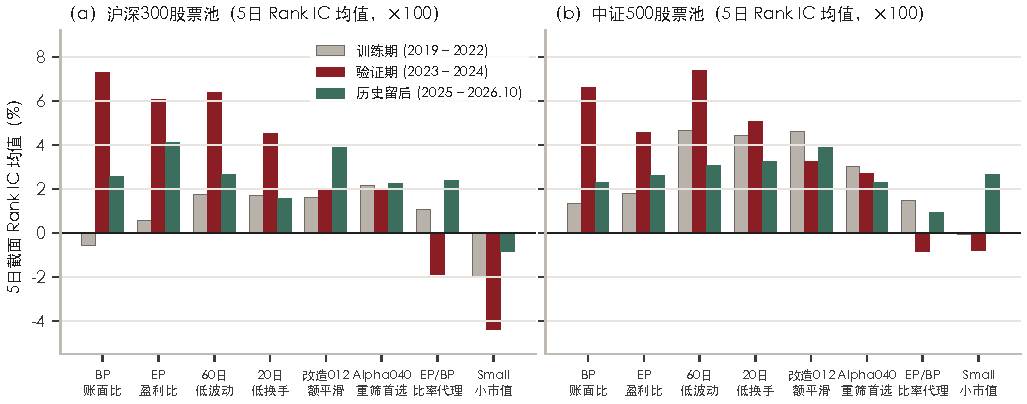
\includegraphics[width=\textwidth]{../figures/report_tex/fig03_factor_ic_dual_pool.pdf}\\[-2pt]
{\color{Primary}\rule{\textwidth}{0.6pt}}\\[2pt]
\exhibitnote{资料来源：Tushare 官方接口与随包申万行业历史表，列祖列宗量化投研部测算。注：纵轴为截面 5 日 Spearman 秩相关系数（Rank IC）日均值乘以 100。}
\end{minipage}
\vspace{5pt}

从单因子分阶段表现可以归纳出三条规律：（1）\textbf{60日低波动与20日低换手在两池三段全部保持正向平均 IC}，且 5 日截面自相关系数稳定在约 0.97--0.98 区间（其中中证500验证期低波动因子为 0.9692），具备支撑低换手周度持仓的信号持续性；在沪深300全样本上，两者日均截面秩相关为 0.574，60日低波动与 BP 的截面秩相关为 0.324，呈中低度正相关而可提供互补信息；（2）\textbf{无量纲成交额平滑改造012在两池三段的单因子平均 IC 全为正值}，但 5 日自相关约为 0.45，换手高于基本面与低风险因子，其能否转化为扣费后净收益须视具体股票池的组合回测而定；（3）\textbf{小市值代理与 EP/BP 比率代理呈现明显跨期或跨池分化}，小市值代理在沪深300三段平均 IC 均为负而在中证500两段为正，由 EP/BP 直接派生的比率代理（与 BP、EP 全期截面秩相关分别为 -0.272 与 +0.281）在验证期两池平均 IC 均为负值（沪深300为 $-0.0187$、中证500为 $-0.0085$）。

\subsection{3.2 次日开盘无前视账户引擎与交叉复算校验}

为使组合回测严格反映真实交易时序，账户引擎在信号日 $t$ 收盘生成目标权重后，统一于下一交易日 $t+1$ 开盘集合竞价后按已知信息执行撮合，并遵守五项制度约束：第一，\textbf{开盘成交许可过滤}，买入标的须同时满足当日正常交易、开盘报价有效且大于零、当日未被实施风险警示（逐日 ST 判定），且开盘相对前收盘涨跌幅未触及板块限价阈值（科创板与创业板 $\pm 19.5\%$、当日 ST 股 $\pm 4.5\%$、其他主板标的 $\pm 9.5\%$）；已调出池或变为 ST 的存量持仓允许在非开盘跌停日正常卖出变现。第二，\textbf{双印花税费率情景并列}，全篇默认主报固定卖出千 1 印花税基准情景（买侧万 3 佣金加千 1 滑点共 13 bp，卖侧千 1 印花税加万 3 佣金加千 1 滑点共 23 bp，双边等额换仓往返成本约 36 bp），同时附列自 2023 年 8 月 28 日起按财政部、税务总局公告将卖出印花税减半至 5 bp 的历史税率情景。第三，\textbf{现金非负与账本零残差闭合}，调仓先执行卖出回笼资金再按可用现金比例执行买入，全部 63 组回测账户逐日现金余额全程非负，每日“股票持仓市值 $+$ 期末现金 $-$ 账户总资产”最大绝对残差精确为 0.0。第四，\textbf{价格指数首日开盘对齐}，对比基准沪深300与中证500价格指数在首日（2023-01-09）同样按开盘价至收盘价计算首日收益（沪深300首日 $+0.36\%$），避免策略按开盘建仓而基准按前收盘起算的起点错位。第五，\textbf{双实现独立复算校验}，两套独立编写的账户代码对 14 项核心策略净值完成逐日交叉核对，累计收益最大偏差为 0.0000 个百分点；唯一存在细微差异的是中证500历史基线 M0b（主净值源为 $-10.96\%$，随包早期参考脚本因保留全期任一时点 ST 过滤而为 $-10.84\%$，相差 0.12 个百分点），在此予以透明备查。

\subsection{3.3 双股票池回测与 M4 选型}

在统一账户引擎下，我们在沪深300与中证500两个股票池上完整回测了历史基线与控制变量消融序列（见图表 9 与图表 10）。回测全期为 2023-01-09 至 2026-10-30（921 个交易日），其中 2023-01-09 至 2024-12-31（480 个交易日）为验证期；2025-01-02 至 2026-10-30（441 个交易日）因在课题多轮方案迭代中已参与讨论与对比，全文统一界定为“历史留后区间”，不作纯样本外盲测宣称。需要特别说明各面板共同池口径：在沪深300面板中，M1、M2、M3b、M4、M5 共享解除 Alpha015 覆盖约束后的干净共同池（调仓日可选股票中位数 284 只），含 Alpha015 的 M3a 留在 3.4 节同池专题对照；在中证500面板中，M0a 与 M0b 沿用历史基线入池口径（185 个信号日中有 85 个信号日 M0a 与 M1 的可选股票集合不同），M1 至 M5 则严格共享同一共同池。

\vspace{4pt}
\noindent\begin{minipage}{\textwidth}
\setlength{\parindent}{0pt}\setlength{\tabcolsep}{3.1pt}
\exhibitcap{图表 9：沪深300与中证500双股票池回测绩效与选型对照表（2023-01-09 至 2026-10-30）}
\fontsize{7.5pt}{10.1pt}\selectfont
\begin{tabularx}{\textwidth}{@{}X r r r r r r r r r@{}}
  \arrayrulecolor{Primary}\toprule[1.0pt]
  \rowcolor{TblHdr}
  \textbf{\sffamily 模型与股票池口径} & \textbf{\sffamily 全期净收益} & \textbf{\sffamily 历史税率} & \textbf{\sffamily 几何年化} & \textbf{\sffamily 年化波动} & \textbf{\sffamily 验证期} & \textbf{\sffamily 历史留后} & \textbf{\sffamily 算术夏普} & \textbf{\sffamily 最大回撤} & \textbf{\sffamily 单次换手} \\
  \rowcolor{TblHdr}
  {\fontsize{6.4}{7.8}\selectfont\textcolor{GrayNote}{（921交易日，未扣产品费）}} &
  {\fontsize{6.4}{7.8}\selectfont\textcolor{GrayNote}{(千1税, \%) }} &
  {\fontsize{6.4}{7.8}\selectfont\textcolor{GrayNote}{(减半税, \%) }} &
  {\fontsize{6.4}{7.8}\selectfont\textcolor{GrayNote}{(\%)}} &
  {\fontsize{6.4}{7.8}\selectfont\textcolor{GrayNote}{(\%)}} &
  {\fontsize{6.4}{7.8}\selectfont\textcolor{GrayNote}{(23--24, \%) }} &
  {\fontsize{6.4}{7.8}\selectfont\textcolor{GrayNote}{(25--26, \%) }} &
  {\fontsize{6.4}{7.8}\selectfont\textcolor{GrayNote}{($r_f=0$)}} &
  {\fontsize{6.4}{7.8}\selectfont\textcolor{GrayNote}{(\%)}} &
  {\fontsize{6.4}{7.8}\selectfont\textcolor{GrayNote}{(\%/次)}} \\
  \midrule[0.5pt]
    \multicolumn{10}{@{}l}{\textbf{\sffamily\textcolor{Primary}{A. 沪深300股票池（历史基线 M0a / M0b；解除 Alpha015 覆盖约束干净共同池消融 M1、M2、M3b、M4、M5）}}}\\[1pt]
    M0a（5日无缓冲历史基线） & +41.56 & +42.18 & +9.98 & 16.03 & +26.82 & +11.62 & 0.673 & -17.02 & 5.83 \\
    M0b（50\%量价高换手对照） & -8.88 & -5.22 & -2.51 & 16.31 & -4.64 & -4.45 & -0.075 & -28.14 & 51.70 \\
    M1（三因子基准，前75缓冲） & +51.11 & +51.36 & +11.96 & 15.74 & +32.47 & +14.07 & 0.796 & -14.76 & 2.35 \\
    M2（纯价值：去规模代理） & +42.99 & +43.14 & +10.28 & 15.51 & +29.24 & +10.64 & 0.709 & -15.95 & 1.59 \\
    M3b（纯价值+15\%改造012） & +51.57 & +51.78 & +12.05 & 15.53 & +32.23 & +14.63 & 0.811 & -16.34 & 1.95 \\
    \textbf{\textcolor{Primary}{M4（主交付：价值低波四因子）}} & \textbf{\textcolor{Primary}{+56.58}} & \textbf{+56.86} & \textbf{+13.05} & \textbf{14.75} & \textbf{+39.54} & \textbf{+12.21} & \textbf{\textcolor{Primary}{0.905}} & \textbf{-15.88} & \textbf{2.74} \\
    M5（五因子对照：M4+EP/BP） & +60.79 & +61.10 & +13.88 & 14.69 & +31.09 & +22.65 & 0.958 & -14.32 & 2.81 \\
    沪深300价格指数（000300.SH） & -0.33 & -0.33 & -0.09 & 17.42 & -1.59 & +1.29 & 0.082 & -24.80 & — \\
    \arrayrulecolor{RuleMuted}\midrule[0.4pt]
    \multicolumn{10}{@{}l}{\textbf{\sffamily\textcolor{Primary}{B. 中证500股票池（历史基线 M0a / M0b；共同池消融 M1 至 M5）}}}\\[1pt]
    M0a（5日无缓冲历史基线） & +29.88 & +30.62 & +7.41 & 19.04 & +17.48 & +10.55 & 0.471 & -22.07 & 7.69 \\
    M0b（50\%量价高换手对照） & -10.96 & -6.97 & -3.13 & 18.97 & -13.28 & +2.68 & -0.073 & -36.57 & 56.39 \\
    M1（三因子基准，前75缓冲） & +36.49 & +36.84 & +8.88 & 18.85 & +17.97 & +15.70 & 0.546 & -21.23 & 3.56 \\
    M2（纯价值：去规模代理） & +47.74 & +48.05 & +11.27 & 17.74 & +20.26 & +22.85 & 0.691 & -20.53 & 2.93 \\
    M3a（90\%基准+10\%重筛Alpha） & +33.09 & +33.52 & +8.14 & 18.73 & +15.32 & +15.42 & 0.511 & -21.82 & 4.28 \\
    M3b（纯价值+15\%改造012） & +40.81 & +41.17 & +9.82 & 17.69 & +17.81 & +19.53 & 0.618 & -20.78 & 3.44 \\
    \textbf{\textcolor{Primary}{M4（跨池对照：价值低波四因子）}} & \textbf{\textcolor{Primary}{+57.73}} & \textbf{+58.22} & \textbf{+13.28} & \textbf{17.07} & \textbf{+35.85} & \textbf{+16.11} & \textbf{\textcolor{Primary}{0.816}} & \textbf{\textcolor{Primary}{-16.46}} & \textbf{4.37} \\
    M5（五因子对照：M4+EP/BP） & +55.17 & +55.69 & +12.77 & 16.93 & +23.61 & +25.54 & 0.795 & -20.21 & 4.63 \\
    中证500价格指数（000905.SH） & +3.94 & +3.94 & +1.06 & 23.43 & -5.02 & +9.44 & 0.162 & -31.15 & — \\
  \arrayrulecolor{Primary}\bottomrule[1.0pt]
\end{tabularx}\\[3pt]
\exhibitnote{资料来源：个股行情、估值、换手率、复权因子与逐日ST源自 Tushare 官方接口；94期月度历史成分、申万一级行业与双价格指数（000300.SH、000905.SH）源自随包历史输入；列祖列宗量化投研部测算。注：1）沪深300原含 Alpha015 共同池（中位数 152 股）内 M1 与 M3a 扣费净收益分别为 -3.44\% 与 -1.83\%，详见 3.4 节；2）组合净值基于后复权价计算（含现金分红），两项对比指数均为价格指数（不含现金分红）；各模型行业持仓集中度详见第四章图表 15。}
\end{minipage}
\vspace{5pt}

\noindent\begin{minipage}{\textwidth}
\setlength{\parindent}{0pt}
\exhibitcap{图表 10：中证500同规格模型累计净值走势与双股票池算术夏普比率对比}
{\color{Primary}\rule{\textwidth}{0.8pt}}\\[2pt]
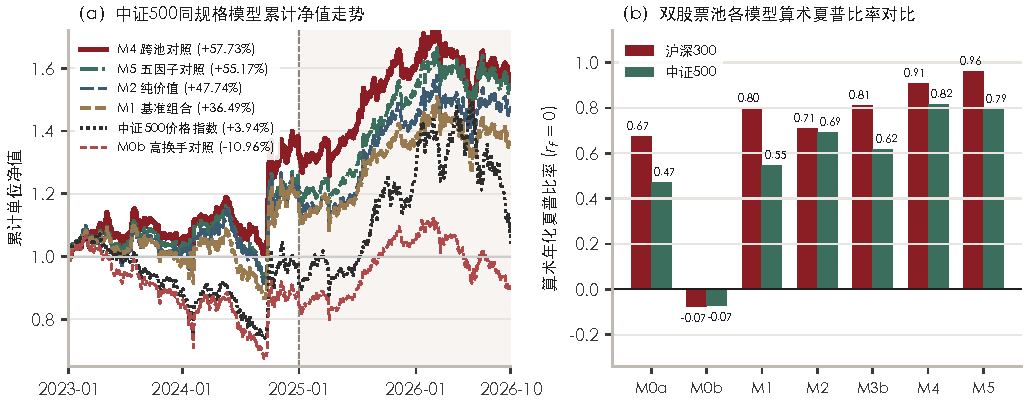
\includegraphics[width=\textwidth]{../figures/report_tex/fig04_dual_pool_nav_and_bars.pdf}\\[-2pt]
{\color{Primary}\rule{\textwidth}{0.6pt}}\\[2pt]
\exhibitnote{资料来源：Tushare 官方接口与随包历史输入，列祖列宗量化投研部测算。注：左图为中证500池固定千1印花税情景净值走势（沪深300净值走势见首页图表 1），右图为双股票池各模型日频算术年化夏普比率（$r_f=0$）对比。}
\end{minipage}
\vspace{5pt}

围绕图表 9 与图表 10 的完整双池证据（包括反例），研究团队对各消融环节与最终选型作出如下四点分析：

第一，\textbf{高换手摩擦损耗与基线演进的归因边界。}在每 5 交易日调仓规则下，引入 50\% 短窗量价因子的 M0b 在沪深300与中证500上单次单边换手分别高达 51.70\% 与 56.39\%，扣费后净收益跌至 -8.88\% 与 -10.96\%，印证了在千 1 印花税与滑点约束下控制换手的必要性。沪深300干净池 M1 较历史基线 M0a 累计净收益高出 +9.55 个百分点（+51.11\% 对 +41.56\%），中证500 M1 亦高于 M0a（+36.49\% 对 +29.88\%）；由于 M1 与 M0a 同时改变了前 75 名保留缓冲带与当期可选股票集合，该差值属于两项规则调整的复合账户差。

第二，\textbf{规模代理与改造动量因子的跨市场结构分化。}剥离小市值代理后，纯价值 M2 在沪深300上因超大盘银行股权重上升，全期净收益由 M1 的 +51.11\% 回落至 +42.99\%；而在中证500中盘池内，剥离小市值代理后 M2 净收益由 +36.49\% 升至 +47.74\%。进一步在纯价值底盘上叠加 15\% 无量纲成交额平滑改造因子（M3b 对照同池 M2），沪深300净收益提升 +8.58 个百分点（+51.57\% 对 +42.99\%），但中证500同配方净收益反而下降 6.93 个百分点（+40.81\% 对 +47.74\%）；中证500上叠加 10\% 重筛 Alpha101 的 M3a 亦较同池 M1 低 3.40 个百分点。这表明单因子平均 IC 为正并不必然转化为跨池一致的扣费组合收益增量。

第三，\textbf{M4 相对 M1 的同池得失权衡。}在沪深300干净共同池内，将小市值代理替换为中性化低波与低换手后，M4 全期累计净收益达 +56.58\%（历史减半税率情景为 +56.86\%），高于 M1 的 +51.11\%，年化波动率由 15.74\% 降至 14.75\%，算术年化夏普由 0.796 升至 0.905，日频信息比率达 0.875。同时主表也如实呈现出两项反向证据：一是 M4 的全期最大回撤（-15.88\%）略深于 M1（-14.76\%）；二是分段回测显示，M4 相对 M1 的收益优势集中在验证期（+39.54\% 对 +32.47\%），历史留后区间则落后于 M1（+12.21\% 对 +14.07\%）。而在中证500池内，M4 相对 M1 的全期净收益提升幅度更大（+57.73\% 对 +36.49\%），最大回撤亦由 -21.23\% 收窄至 -16.46\%。

第四，\textbf{M4 与五因子 M5 的跨池选型取舍。}单看沪深300股票池，五因子模型 M5 的全期净收益（+60.79\%）、算术夏普（0.958）与最大回撤（-14.32\%）三项指标均优于 M4。但把完全相同的两套公式用于中证500股票池后，排序发生反转：中证500 M4 在全期净收益（+57.73\% 对 +55.17\%）、算术夏普（0.816 对 0.795）与最大回撤（-16.46\% 对 -20.21\%）上全面优于 M5，并居该池八个模型首位。结合第四章归因结果（EP/BP 比率代理在中证500横截面归因中呈 -2.90 个百分点/年的负向拖累，在沪深300仅贡献 +0.14 个百分点/年），不纳入该项来减少一个由 EP/BP 直接派生的比率因子，能够在双股票池之间获得更一致的稳健表现。综合跨池一致性与模型简洁性，团队选定 \textbf{沪深300 M4} 作为私募产品化主交付模型。

\subsection{3.4 专题分析：Alpha015 低覆盖约束对共同选股池与组合换手的传导机制}

在沪深300初始联合消融阶段，若要求全部候选模型（M1 至 M5）在包含重筛第三席 Alpha015 的总交集池上选股，所有低换手设计模型的单次单边换手均异常飙升至 41\% 以上，扣费净收益跌至负值或个位数。为厘清这一现象究竟源于因子打分失效还是共同池资格收缩，我们对原含 Alpha015 共同池中的 M1 调仓退出记录进行了逐笔穿透核查（见图表 11 与图表 12）。

\vspace{4pt}
\noindent\begin{minipage}{\textwidth}
\setlength{\parindent}{0pt}\setlength{\tabcolsep}{3.8pt}
\exhibitcap{图表 11：沪深300原含 Alpha015 共同池（M1 / M3a）与解除覆盖约束干净池（M1）诊断表}
\fontsize{7.8pt}{10.6pt}\selectfont
\begin{tabularx}{\textwidth}{@{}X r r r r r r r@{}}
  \arrayrulecolor{Primary}\toprule[1.0pt]
  \rowcolor{TblHdr}
  \textbf{\sffamily 沪深300共同池约束与评分对照} & \textbf{\sffamily 共同池中位数} & \textbf{\sffamily 目标替换率} & \textbf{\sffamily 全期毛收益} & \textbf{\sffamily 千1税净收益} & \textbf{\sffamily 算术夏普} & \textbf{\sffamily 单次换手} & \textbf{\sffamily 累计成本拖累} \\
  \midrule[0.5pt]
  原含 Alpha015 共同池 M1 & 152 股 & 41.18\% & +27.58\% & -3.44\% & 0.032 & 41.91\% & 27.34\% \\
  原含 Alpha015 共同池 M3a & 152 股 & 41.39\% & +30.28\% & -1.83\% & 0.057 & 42.58\% & 27.82\% \\
  \textbf{\textcolor{Primary}{解除 Alpha015 约束干净池 M1}} & \textbf{284 股} & \textbf{1.03\%} & \textbf{+53.41\%} & \textbf{\textcolor{Primary}{+51.11\%}} & \textbf{0.796} & \textbf{2.35\%} & \textbf{1.87\%} \\
  \arrayrulecolor{Primary}\bottomrule[1.0pt]
\end{tabularx}\\[3pt]
\exhibitnote{资料来源：覆盖率退出审计表与统一账户回测账本，列祖列宗量化投研部测算。注：M1 本身完全不使用 Alpha015 打分；同池内 M3a（90\% M1 得分 + 10\% 入选三项 Alpha）相对含 015 池 M1 净收益差为 +1.62 个百分点。}
\end{minipage}
\vspace{5pt}

\noindent\begin{minipage}{\textwidth}
\setlength{\parindent}{0pt}
\exhibitcap{图表 12：沪深300同一 M1 评分公式在不同共同池约束下的净值走势与单次换手率对比}
{\color{Primary}\rule{\textwidth}{0.8pt}}\\[2pt]
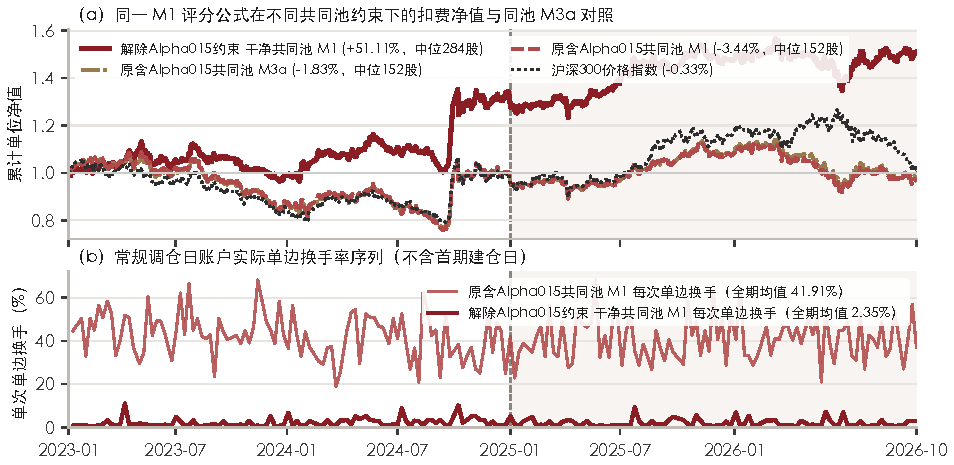
\includegraphics[width=\textwidth]{../figures/report_tex/fig05_alpha015_coverage_diag.pdf}\\[-2pt]
{\color{Primary}\rule{\textwidth}{0.6pt}}\\[2pt]
\exhibitnote{资料来源：Tushare 官方接口与账户回测调仓明细，列祖列宗量化投研部测算。}
\end{minipage}
\vspace{5pt}

穿透审计表明：在首期建仓后的 184 次常规调仓中，原含 Alpha015 共同池 M1 累计退出的 3,789 个持仓席位里，有 3,605 次（占比 95.1\%）完全满足可交易及 M1 自身所需三因子（BP、EP、Small）非空条件，仅因当日缺失短窗因子 Alpha015 而丧失共同池资格、被迫清仓换股。解除该项不相关的入池交集约束后，调仓日共同池规模中位数由 152 只恢复至 284 只，同一 M1 公式的目标持仓替换率由 41.18\% 降至 1.03\%，账户实际平均单次单边换手由 41.91\% 降至 2.35\%。

值得强调的是，解除覆盖约束后 M1 的无交易费毛收益同步由 +27.58\% 升至 +53.41\%，扣费净收益由 -3.44\% 升至 +51.11\%；而在原含 Alpha015 的同一共同池内，叠加 10\% 重筛 Alpha 的 M3a 较 M1 净收益仅相差 +1.62 个百分点。这说明低覆盖率因子进入多模型共同池交集会产生双重扭曲：一方面改变基准组合原本的持股集合导致毛收益变形，另一方面令前 75 名保留缓冲带形同虚设并引发高额换手摩擦。将干净共同池主消融（M1、M2、M3b、M4、M5）与含 Alpha015 同池对照（M3a 对照 M1）分列披露，能够准确剥离覆盖率约束效应与打分增量效应。

% =========================================================================
% 四、横截面收益归因与多维风险分析
% =========================================================================
\section{四、横截面收益归因与多维风险分析}

\subsection{4.1 隔夜盘中账本分解与滞后持仓横截面回归归因}

在精确闭合的日频账户账本上，组合总净收益首先可按交易时段分解为隔夜收益（前收盘至当日开盘）、盘中收益（当日开盘至收盘）与交易成本三部分：在 921 个交易日内，沪深300 M4 累计盘中收益贡献为 +79.06\%，隔夜收益变动为 -20.22\%，交易成本直接消耗为 2.26\%（三项复利合成精确等于累计净收益 +56.58\%）；中证500 M4 盘中贡献为 +62.11\%，隔夜变动为 -0.69\%，交易成本消耗为 3.70\%。需要指出，由于 A 股市场指数本身存在显著的隔夜负收益与盘中正收益日内结构特征，上述盘中累计贡献同时包含市场基准与行业整体的日内波动，不能直接等同于个股纯选股超额；账本分解的明确结论在于，排名缓冲机制将近四年全周期的直接交易摩擦损耗控制在了 2\% 至 4\% 区间。

为进一步拆解组合持仓在不同系统性风格上的收益贡献，我们采用滞后实际持仓的 Fama-MacBeth（1973）横截面回归归因框架：在每个交易日 $t$，以成分股当日总收益对 $t-1$ 日收盘已知的 7 项标准化候选因子（含 BP、EP、60日低波、20日低换手、小市值代理、EP/BP 比率代理及无量纲成交额平滑改造012）执行带截距横截面回归，得到当日市场截距项与各因子纯收益率，再乘以组合当日开盘实际持仓权重向量，经日度加总折算为算术年化收益贡献（见图表 13 与图表 14，全部 10 项分项之和与账户实际算术年化净收益的闭合误差小于 $10^{-10}$）。

\vspace{4pt}
\noindent\begin{minipage}{\textwidth}
\setlength{\parindent}{0pt}\setlength{\tabcolsep}{3.5pt}
\exhibitcap{图表 13：双股票池核心模型滞后实际持仓 7 因子 Fama-MacBeth 算术年化收益归因表}
\fontsize{7.7pt}{10.5pt}\selectfont
\begin{tabularx}{\textwidth}{@{}X r r r r r r@{}}
  \arrayrulecolor{Primary}\toprule[1.0pt]
  \rowcolor{TblHdr}
  \textbf{\sffamily 归因分项（算术年化，百分点/年）} & \textbf{\sffamily 沪深300 M1} & \textbf{\sffamily 沪深300 M4} & \textbf{\sffamily 沪深300 M5} & \textbf{\sffamily 中证500 M1} & \textbf{\sffamily 中证500 M4} & \textbf{\sffamily 中证500 M5} \\
  \midrule[0.5pt]
    市场截距项（截面等权基准收益） & +4.46 & +4.46 & +4.46 & +6.46 & +6.46 & +6.46 \\
    账面市值比（BP）暴露贡献 & +4.09 & +4.03 & +3.71 & -1.15 & -1.09 & -0.41 \\
    盈利收益率（EP）暴露贡献 & +2.40 & +2.43 & +2.38 & +6.40 & +5.96 & +6.90 \\
    \textbf{60日低波动（LowVol60）暴露贡献} & +0.93 & \textbf{\textcolor{Primary}{+1.62}} & +1.36 & +1.09 & \textbf{\textcolor{Primary}{+2.17}} & +1.94 \\
    \textbf{20日低换手（LowTurn20）暴露贡献} & +0.28 & \textbf{\textcolor{Primary}{+0.87}} & +0.86 & +0.71 & \textbf{\textcolor{Primary}{+0.84}} & +0.62 \\
    小市值代理（Small）暴露贡献 & +0.18 & +0.54 & +0.46 & -0.26 & +0.08 & +0.72 \\
    隐含账面盈利率代理（EP/BP）贡献 & -0.03 & -0.26 & +0.14 & -1.16 & +0.03 & -2.90 \\
    无量纲成交额平滑改造012暴露贡献 & +0.17 & -0.18 & -0.02 & +0.15 & +0.25 & +0.21 \\
    特异残差与调仓择时项 & +0.47 & +0.32 & +1.23 & -1.33 & +0.01 & +0.74 \\
    交易成本直接拖累 & -0.41 & -0.49 & -0.50 & -0.63 & -0.78 & -0.83 \\
    \arrayrulecolor{RuleMuted}\midrule[0.4pt]
    \textbf{账户实际算术年化净收益（闭合对账）} & +12.54 & \textbf{\textcolor{Primary}{+13.36}} & +14.08 & +10.28 & \textbf{\textcolor{Primary}{+13.92}} & +13.45 \\
  \arrayrulecolor{Primary}\bottomrule[1.0pt]
\end{tabularx}\\[3pt]
\exhibitnote{资料来源：滞后标准化因子矩阵与实际开盘持仓矩阵，列祖列宗量化投研部测算。注：即使某模型未在选股打分中使用某项因子，只要其持仓在该因子上存在非零横截面暴露，7因子多元回归仍会忠实记录对应暴露收益。}
\end{minipage}
\vspace{5pt}

\noindent\begin{minipage}{\textwidth}
\setlength{\parindent}{0pt}
\exhibitcap{图表 14：沪深300与中证500组合（M4 对照 M5 / M1）算术年化收益归因分解图}
{\color{Primary}\rule{\textwidth}{0.8pt}}\\[2pt]
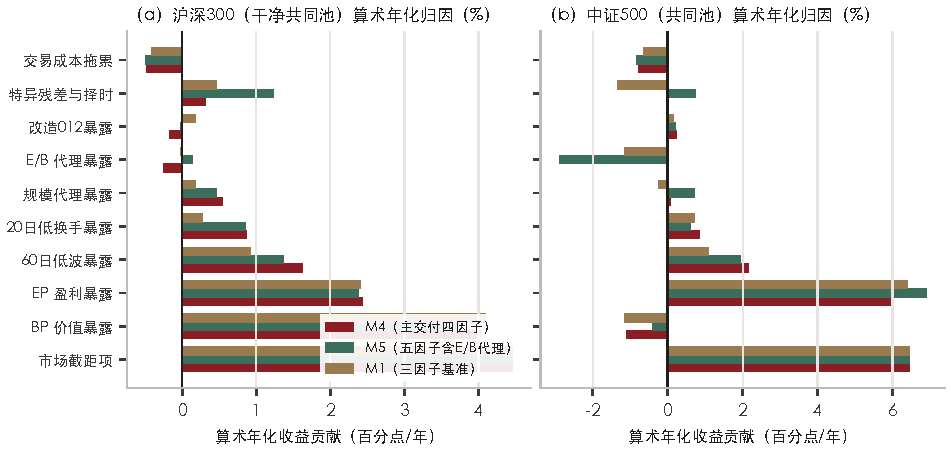
\includegraphics[width=\textwidth]{../figures/report_tex/fig06_fm_attribution_dual_pool.pdf}\\[-2pt]
{\color{Primary}\rule{\textwidth}{0.6pt}}\\[2pt]
\exhibitnote{资料来源：列祖列宗量化投研部测算。注：横轴为固定千1印花税基准情景下各归因分项的算术年化贡献（百分点/年）。}
\end{minipage}
\vspace{5pt}

横截面归因表提供了两项核心经验证据：第一，在该 7 因子横截面回归设定下，沪深300 M4 中 60 日低波动与 20 日低换手两项防御暴露合计贡献 +2.49 个百分点/年（其中低波 +1.62\%、低换手 +0.87\%），较同池基准 M1 高出 $+1.28$ 个百分点/年；在中证500 M4 中，两项低风险因子合计贡献 +3.01 个百分点/年（低波 +2.17\%、低换手 +0.84\%）。同时，M4 在沪深300与中证500上的特异残差与择时项年化均值分别为 +0.32\% 与 +0.01\%，说明历史期间组合收益主要可由模型显式纳入的价值与低风险截面暴露予以解释（但需注意，残差全期均值较小不代表其逐日波动可忽略，也不构成未来收益稳定性的保证）。第二，对比 M5 与 M4 可见，新增的 EP/BP 比率代理在沪深300 M5 中直接暴露贡献仅为 +0.14 个百分点/年，M5 高出 M4 的部分较多体现于特异残差项（+1.23\%）；而在中证500 M5 中，该比率代理暴露直接带来 -2.90 个百分点/年的负贡献。这一归因结构从收益来源层面佐证了 3.3 节放弃该派生比率、选定四因子 M4 的合理性。

\subsection{4.2 申万一级行业暴露结构与水下回撤分析}

由于 M4 对账面市值比（BP）与盈利收益率（EP）保留了原始跨行业比价而不做行业中性化，组合在低估值大金融板块上的持仓集中度是需要直接量化披露的核心风险点。图表 15 与图表 16 报告了各代表性组合在申万一级行业上的全期平均开盘持仓权重与期末（2026-10-30）截面持仓权重。

\vspace{4pt}
\noindent\begin{minipage}{\textwidth}
\setlength{\parindent}{0pt}\setlength{\tabcolsep}{3.8pt}
\exhibitcap{图表 15：双股票池核心模型申万一级行业持仓权重与金融板块集中度核查表}
\fontsize{7.8pt}{10.6pt}\selectfont
\begin{tabularx}{\textwidth}{@{}X r r r r r r@{}}
  \arrayrulecolor{Primary}\toprule[1.0pt]
  \rowcolor{TblHdr}
  \textbf{\sffamily 组合与股票池} & \textbf{\sffamily 银行} & \textbf{\sffamily 非银金融} & \textbf{\sffamily 金融合计} & \textbf{\sffamily 交通运输} & \textbf{\sffamily 建筑装饰} & \textbf{\sffamily 公用事业} \\
  \rowcolor{TblHdr}
  {\fontsize{6.5}{8}\selectfont\textcolor{GrayNote}{（实际开盘持仓权重，\%）}} &
  {\fontsize{6.5}{8}\selectfont\textcolor{GrayNote}{(均值/期末)}} &
  {\fontsize{6.5}{8}\selectfont\textcolor{GrayNote}{(均值/期末)}} &
  {\fontsize{6.5}{8}\selectfont\textcolor{GrayNote}{(均值/期末)}} &
  {\fontsize{6.5}{8}\selectfont\textcolor{GrayNote}{(全期均值)}} &
  {\fontsize{6.5}{8}\selectfont\textcolor{GrayNote}{(全期均值)}} &
  {\fontsize{6.5}{8}\selectfont\textcolor{GrayNote}{(全期均值)}} \\
  \midrule[0.5pt]
    沪深300 M0a（历史基线） & 34.2 / 32.0 & 4.4 / 28.0 & 38.6 / 60.0 & 5.5 & 13.4 & 2.6 \\
    沪深300 M1（三因子基准） & 35.1 / 40.0 & 3.7 / 12.0 & 38.8 / 52.0 & 6.0 & 13.2 & 2.7 \\
    沪深300 M2（去规模纯价值） & 41.3 / 48.0 & 6.8 / 18.0 & 48.2 / 66.0 & 6.0 & 12.3 & 1.0 \\
    \textbf{\textcolor{Primary}{沪深300 M4（旗舰主交付）}} & \textbf{37.2 / 42.0} & \textbf{5.2 / 8.0} & \textbf{\textcolor{Primary}{42.4 / 50.0}} & \textbf{5.4} & \textbf{9.3} & \textbf{0.1} \\
    沪深300 M5（五因子对照） & 37.8 / 44.0 & 5.6 / 8.0 & 43.4 / 52.0 & 4.8 & 9.1 & 1.2 \\
    \arrayrulecolor{RuleMuted}\midrule[0.35pt]
    中证500 M4（跨池同规格对照） & 16.5 / 10.0 & 5.8 / 8.0 & 22.3 / 18.0 & 6.1 & 3.6 & 6.4 \\
  \arrayrulecolor{Primary}\bottomrule[1.0pt]
\end{tabularx}\\[3pt]
\exhibitnote{资料来源：逐日开盘实际持仓矩阵与随包申万一级行业映射表，列祖列宗量化投研部测算。注：“金融合计”定义为申万一级“银行”与“非银金融”两行业持仓权重之和；期末指回测截止日 2026-10-30。}
\end{minipage}
\vspace{5pt}

\noindent\begin{minipage}{\textwidth}
\setlength{\parindent}{0pt}
\exhibitcap{图表 16：申万一级行业平均持仓暴露与双池金融集中度对比图}
{\color{Primary}\rule{\textwidth}{0.8pt}}\\[2pt]
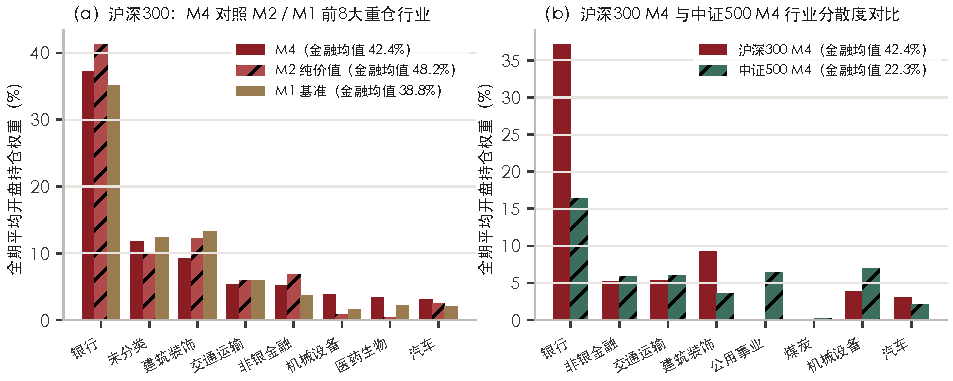
\includegraphics[width=\textwidth]{../figures/report_tex/fig07_industry_exposure.pdf}\\[-2pt]
{\color{Primary}\rule{\textwidth}{0.6pt}}\\[2pt]
\exhibitnote{资料来源：列祖列宗量化投研部测算。}
\end{minipage}
\vspace{5pt}

行业核查显示两方面特征：一方面，与单纯去掉规模因子的纯价值组合 M2（金融板块全期均值 48.2\%、期末 66.0\%）及历史基线 M0a（期末金融权重 60.0\%）相比，引入经行业中性化处理的低波动与低换手因子后，沪深300 M4 的金融板块权重回落至全期均值 42.4\%、期末 50.0\%（其中银行股全期均值 37.2\%、期末 42.0\%），其余仓位分散配置于交通运输、建筑装饰、公用事业与煤炭等现金流稳健板块；在中证500池内，M4 的金融持仓进一步降至全期均值 22.3\%、期末 18.0\%，说明四因子框架在中盘池并不依赖金融行业贡献收益。另一方面，沪深300 M4 高达四至五成的金融板块权重在绝对水平上仍属偏高集中暴露，一旦市场切换至高弹性科技成长单边领涨、红利与大金融相对滞涨的阶段（如历史留后区间部分时段），组合相对宽基指数及均衡型策略会出现阶段性跑输。

\vspace{4pt}
\noindent\begin{minipage}{\textwidth}
\setlength{\parindent}{0pt}
\exhibitcap{图表 17：核心组合与市场价格指数动态水下回撤曲线（2023-01-09 至 2026-10-30）}
{\color{Primary}\rule{\textwidth}{0.8pt}}\\[2pt]
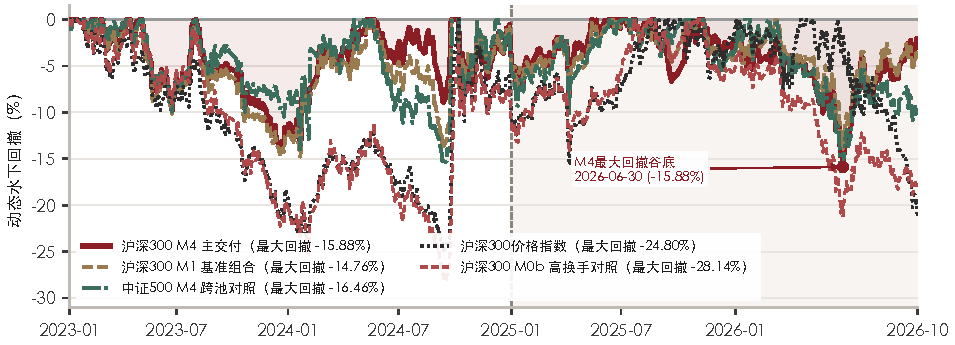
\includegraphics[width=\textwidth]{../figures/report_tex/fig08_underwater_drawdown.pdf}\\[-2pt]
{\color{Primary}\rule{\textwidth}{0.6pt}}\\[2pt]
\exhibitnote{资料来源：列祖列宗量化投研部测算。注：水下回撤按当日累计单位净值相对此前历史最高单位净值（不低于初始值 1.0000）的跌幅计算。}
\end{minipage}
\vspace{5pt}

在水下回撤与净值轨迹维度（图表 17），须严格区分“单位净值历史最低点”与“峰值至谷底最大回撤”两项不同概念：在固定千 1 印花税基准情景下，沪深300 M4 自 2023 年 1 月 9 日以初始净值 1.0000 运作以来，全期最低单位净值为 \textbf{0.9926}（发生于建仓首周 2023-01-12），此后单位净值全程运行于面值上方；全期最大回撤 \textbf{-15.88\%} 则发生于组合前期累积较大涨幅之后，对应单位净值由 2025-11-12 的阶段峰值 \textbf{1.5999} 回落至 2026-06-30 的阶段谷底 \textbf{1.3458}。横向比较来看，沪深300 M4 的最大回撤较同期沪深300价格指数（-24.80\%）浅 8.92 个百分点，较 M0b 高换手对照（-28.14\%）浅 12.26 个百分点，全期年化波动率亦控制在 14.75\%（同期价格指数为 17.42\%）。

% =========================================================================
% 五、私募产品方案、容量情景与雪球模拟跟踪
% =========================================================================
\section{五、私募产品方案、容量情景与雪球模拟跟踪}

\subsection{5.1 产品要素、拟议风控条款与客户分层定位}

围绕沪深300 M4 纯多头、低换手、高蓝筹流动性与清晰因子暴露的特征，我们将策略转化为私募证券投资基金产品方案“沪深300价值低波精选量化私募证券投资基金（M4）”。产品拟设月度开放申赎、单笔份额 6 个月硬锁定期，以匹配周度低换手组合的资金属性，减少短期频繁申赎造成的被动现金摩擦。

在风控条款设计上，结合 4.2 节对单位净值极值与行业暴露的实证核查，区分两类条款口径：其一，\textbf{单位净值预警线与止损线}，拟议设定基金单位净值 \textbf{0.85 为预警线}（触及后在 5 个交易日内将权益仓位上限降至 50\%）、\textbf{0.80 为止损线}（触及后变现权益资产转入高等级货币管理工具）。需要明确说明，历史回测中单位净值最低值为 0.9926，最大回撤 -15.88\% 发生于高净值区间（1.5999 至 1.3458），未曾触及 0.85 或 0.80 阈值；但若实盘产品在高位开放新资金申购，或按新发基金面值 1.00 恰逢同等幅度回撤（跌至约 0.8412），则存在触及 0.85 预警线的真实可能。其二，\textbf{行业集中度约束}，针对沪深300 M4 金融板块全期均值 42.4\%、期末 50.0\% 的集中暴露，拟议在面向机构资金的定制专户合同中增设“申万一级单行业持仓上限 35\%”约束条款。上述 0.85/0.80 净值线与 35\% 单行业上限均属\textbf{拟议产品合同风控条款，未纳入第三章与第四章的历史回测引擎}；若在实盘专户启用单行业上限，需通过带线性约束的组合优化器单独重算历史回测轨迹。

\vspace{4pt}
\noindent\begin{minipage}{\textwidth}
\setlength{\parindent}{0pt}\setlength{\tabcolsep}{3.8pt}
\exhibitcap{图表 18：市场主流大盘权益策略类型定位对比与本产品拟议份额要素表}
\fontsize{7.6pt}{10.3pt}\selectfont
\begin{tabularx}{\textwidth}{@{}l l l X@{}}
  \arrayrulecolor{Primary}\toprule[1.0pt]
  \multicolumn{4}{@{}l}{\textbf{\sffamily\textcolor{Primary}{A. 市场主流沪深300权益产品类型与本策略机制特征定性对比}}}\\[1pt]
  \rowcolor{TblHdr}
  \textbf{\sffamily 策略/产品类型} & \textbf{\sffamily 收益来源与选股方式} & \textbf{\sffamily 换手与费率特征} & \textbf{\sffamily 核心优势与主要适用局限} \\
  \midrule[0.5pt]
  被动沪深300指数ETF & 完全复制市值加权指数 & 换手极低；管理+托管约0.20\% & 费率透明容量大，但弱市需承担完整指数回撤 \\
  中高频量价指增私募 & 多周期高频量价机器学习 & 年化单边常达数十倍；约1\%+20\% & 超额弹性较强，但依赖算力且易受流动性与成本冲击 \\
  主动价值红利公募 & 基金经理基本面深度选股 & 换手偏低；固定费率约1.40\% & 逻辑直观，但持仓风格受投研人员变更与主观判断影响 \\
  \textbf{\textcolor{Primary}{本产品（价值低波M4）}} & \textbf{四因子等权+前75缓冲} & \textbf{单次换手2.74\%；机构C档0.75\%+15\%} & \textbf{规则透明可复现、下行回撤较浅，强成长牛市弹性偏温和} \\
  \arrayrulecolor{RuleMuted}\midrule[0.4pt]
  \multicolumn{4}{@{}l}{\textbf{\sffamily\textcolor{Primary}{B. 本私募基金拟议份额分类、费率结构与目标合格投资者匹配表}}}\\[1pt]
  \rowcolor{TblHdr}
  \textbf{\sffamily 份额类别} & \textbf{\sffamily 目标合格投资者群体} & \textbf{\sffamily 拟议费率与计提方式} & \textbf{\sffamily 起投门槛、流动性安排与风控适用条款} \\
  \midrule[0.4pt]
  A 类标准份额 & 高净值个人客户（绝对收益导向） & 1.00\%管理+0.20\%托管+绝对收益高水位20\% & 100万元起投；月度开放、6个月锁定期；适用0.85预警/0.80止损拟议条款 \\
  B 类超额份额 & 家族办公室及权益配置型个人 & 1.00\%管理+0.20\%托管+相对指数超额20\% & 300万元起投；仅在跑赢沪深300价格指数且创超额新高时计提业绩报酬 \\
  \textbf{\textcolor{Primary}{C 类机构份额}} & \textbf{FOF/MOM、信托及理财子专户} & \textbf{0.60\%管理+0.15\%托管+相对指数超额15\%} & \textbf{1,000万元起投；低固定费率与温和超额分润，可选配单行业 $\le 35\%$ 专户约束} \\
  D 类纯管理费 & 费率透明型机构与长期配置资金 & 1.50\%管理+0.20\%托管，不计提业绩报酬 & 1,000万元起投；消除业绩报酬期权凸性干扰，净值波动路径与原策略一致 \\
  \arrayrulecolor{Primary}\bottomrule[1.0pt]
\end{tabularx}\\[3pt]
\exhibitnote{资料来源：列祖列宗量化投研部依据国内公私募产品通行机制整理。注：面板 A 仅做客观策略机制比较，不引用未经统一回测核验的外部产品历史收益率；面板 B 中预警/止损及专户单行业上限条款未嵌入前期无约束历史回测。}
\end{minipage}
\vspace{5pt}

\subsection{5.2 四档高水位法费后历史模拟净值测算}

在已扣除交易佣金、滑点与固定千 1 印花税的策略净值序列基础上，我们进一步按日计提固定管理费与托管运营费，并按逐日高水位暂提估值（Mark-to-Market）结合自然年末（2023-12-29、2024-12-31、2025-12-31）及回测期末（2026-10-30）结晶扣减规则，模拟测算 A、B、C、D 四类份额投资者的历史费后表现（见图表 19 与图表 20）。

\vspace{4pt}
\noindent\begin{minipage}{\textwidth}
\setlength{\parindent}{0pt}\setlength{\tabcolsep}{2.4pt}
\exhibitcap{图表 19：沪深300 M4 四档高水位法产品费率下历史模拟费后绩效表}
\fontsize{7.25pt}{9.9pt}\selectfont
\begin{tabularx}{\textwidth}{@{}l c >{\raggedright\arraybackslash}X r r r r r r r@{}}
  \arrayrulecolor{Primary}\toprule[1.0pt]
  \rowcolor{TblHdr}
  \textbf{\sffamily 费率方案} & \textbf{\sffamily 固定费率} & \textbf{\sffamily 业绩报酬计提基准} & \textbf{\sffamily 期末净值} & \textbf{\sffamily 累计收益} & \textbf{\sffamily 几何年化} & \textbf{\sffamily 算术夏普} & \textbf{\sffamily 最大回撤} & \textbf{\sffamily 信息比率} & \textbf{\sffamily 年化拖累} \\
  \rowcolor{TblHdr}
  {\fontsize{6.2}{7.6}\selectfont\textcolor{GrayNote}{（千1印花税底盘）}} &
  {\fontsize{6.2}{7.6}\selectfont\textcolor{GrayNote}{(管+托,\%)}} &
  {\fontsize{6.2}{7.6}\selectfont\textcolor{GrayNote}{（年度高水位结晶）}} &
  {\fontsize{6.2}{7.6}\selectfont\textcolor{GrayNote}{(元)}} &
  {\fontsize{6.2}{7.6}\selectfont\textcolor{GrayNote}{(\%)}} &
  {\fontsize{6.2}{7.6}\selectfont\textcolor{GrayNote}{(\%)}} &
  {\fontsize{6.2}{7.6}\selectfont\textcolor{GrayNote}{($r_f=0$)}} &
  {\fontsize{6.2}{7.6}\selectfont\textcolor{GrayNote}{(\%)}} &
  {\fontsize{6.2}{7.6}\selectfont\textcolor{GrayNote}{(vs指数)}} &
  {\fontsize{6.2}{7.6}\selectfont\textcolor{GrayNote}{(pct/年)}} \\
  \midrule[0.5pt]
    策略净值（未扣产品费） & 0.00+0.00 & 无业绩报酬（已含交易费） & 1.5658 & +56.58 & +13.05 & 0.905 & -15.88 & 0.875 & 0.00 \\
    方案 A（标准份额） & 1.00+0.20 & 绝对收益高水位 × 20\% & 1.3918 & +39.18 & +9.47 & 0.763 & -15.99 & 0.622 & 3.58 \\
    方案 B（超额份额） & 1.00+0.20 & 相对价格指数超额 × 20\% & 1.3876 & +38.76 & +9.38 & 0.685 & -16.48 & 0.669 & 3.67 \\
    \textbf{\textcolor{Primary}{方案 C（机构份额）}} & \textbf{0.60+0.15} & \textbf{相对价格指数超额 × 15\%} & \textbf{1.4351} & \textbf{\textcolor{Primary}{+43.51}} & \textbf{\textcolor{Primary}{+10.39}} & \textbf{0.748} & \textbf{-16.26} & \textbf{0.730} & \textbf{2.66} \\
    方案 D（纯管理费） & 1.50+0.20 & 无业绩报酬 & 1.4714 & +47.14 & +11.15 & 0.790 & -16.73 & 0.750 & 1.91 \\
  \arrayrulecolor{Primary}\bottomrule[1.0pt]
\end{tabularx}\\[3pt]
\exhibitnote{资料来源：四档高水位法产品费率测算账本，列祖列宗量化投研部测算。注：方案 B 与方案 C 的超额业绩报酬计提对比基准均为首日开盘对齐的沪深300价格指数（000300.SH，不含分红）；“年化拖累”指未扣产品费几何年化（13.05\%）与扣除产品费后几何年化之差（单位：百分点/年）。}
\end{minipage}
\vspace{5pt}

\noindent\begin{minipage}{\textwidth}
\setlength{\parindent}{0pt}
\exhibitcap{图表 20：四档产品费率方案下投资者历史模拟单位净值走势}
{\color{Primary}\rule{\textwidth}{0.8pt}}\\[2pt]
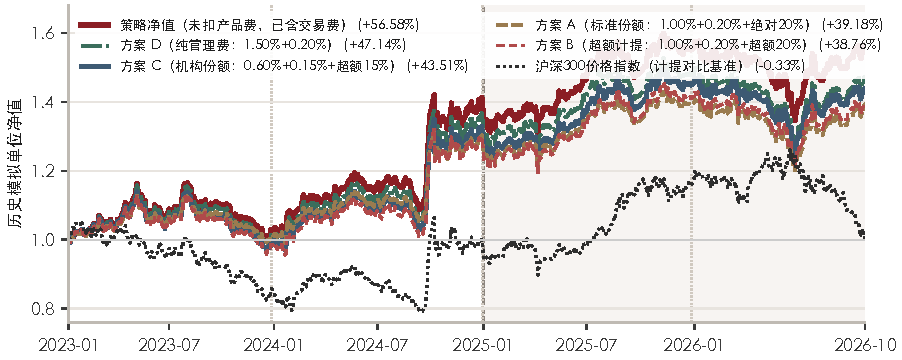
\includegraphics[width=\textwidth]{../figures/report_tex/fig09_fee_hwm_nav.pdf}\\[-2pt]
{\color{Primary}\rule{\textwidth}{0.6pt}}\\[2pt]
\exhibitnote{资料来源：列祖列宗量化投研部测算。注：图中竖向细虚线标示自然年末业绩报酬高水位结晶扣减时点（2023-12-29、2024-12-31、2025-12-31）。}
\end{minipage}
\vspace{5pt}

历史模拟费后结果呈现出清晰的份额特征。面向机构专户与 FOF 资金的\textbf{方案 C（机构份额）}在扣除双层固定费用与相对沪深300价格指数 15\% 超额业绩报酬后，期末历史模拟净值为 1.4351，累计费后净收益 +43.51\%，扣除产品费用后的历史模拟几何年化收益为 \textbf{+10.39\%}（算术夏普 0.748，信息比率 0.730），产品层年化总费率拖累为 \textbf{2.66 个百分点}。不设业绩报酬的\textbf{方案 D（纯管理费份额）}历史模拟费后年化为 +11.15\%（年化拖累 1.91 个百分点）。

值得从机制上解释的是\textbf{方案 A（绝对收益高水位 20\%）与方案 B（相对价格指数超额高水位 20\%）的费后排序}：尽管沪深300价格指数全期累计下跌 -0.33\%，单凭指数全期涨跌幅并不能直接推出两档方案的费后高低，真正的差异来自\textbf{逐年高水位结晶计提时点与复利基数效应}。逐年结晶账本显示，2023 年沪深300价格指数显著下跌而策略小幅正收益，致使在首个结晶日（2023-12-29），按相对超额计提的方案 B 单次结晶扣减了 0.0321 元业绩报酬（结晶后单位净值降至 0.9867），而按绝对收益计提的方案 A 仅结晶扣减 0.0038 元（结晶后净值为 1.0151）。方案 B 在 2023 年末提前流出的这部分本金不再参与 2024 年大涨行情的复利累积，因此即便全周期方案 A 累计实付业绩报酬名义金额（0.0982 元）略高于方案 B（0.0920 元），方案 A 期末到手净值（1.3918，几何年化 +9.47\%）仍略高于方案 B（1.3876，几何年化 +9.38\%）。同时，方案 B 与方案 C 因当前回测数据包仅含价格指数，若实盘专户合同改用沪深300全收益指数作为超额计提基准，管理人业绩报酬提取额将下降、投资者费后留存收益将相应提高。

\subsection{5.3 底层流动性画像与多规模容量执行情景压测}

低换手率本身并不足以直接等同于大资金容量，组合的实际承载规模取决于最难成交的尾部低流动性持仓、单日成交参与率上限以及大额订单的市场冲击成本。我们严格采用调仓日前 20 个交易日无前视日均成交额（$\text{ADV20}_i$）与日收益波动率（$\sigma_{20,i}$），从底层流动性分布、5\% 成交参与率逐期压力测试与平方根市场冲击模型（$\Delta p_i / p_i = Y \cdot \sigma_{20,i} \sqrt{Q_i / \text{ADV20}_i}$，考察 $Y \in \{0.5, 0.8, 1.0\}$）三个维度评估双股票池 M4 的容量边界（见图表 21 与图表 22）。

在底层个股流动性与 P10 容量分位数上，沪深300 M4 全部 185 期持仓标的的 $\text{ADV20}$ 第 10 分位数（P10）与中位数分别为 \textbf{1.59 亿元与 4.64 亿元}，在 5\% 日均成交参与率上限下，单日完成调仓、假设 3 日均分拆单与 5 日变现全部持仓的 P10 容量指标分别为 \textbf{3.33 亿元、9.99 亿元与 6.63 亿元}（中位数分别为 17.96、53.88 与 10.93 亿元）；同规格中证500 M4 持仓标的 $\text{ADV20}$ 的 P10 与中位数仅为 0.59 亿元与 1.45 亿元，对应三项 5\% 参与率 P10 容量分别为 \textbf{1.09 亿元、3.27 亿元与 2.64 亿元}，约为沪深300池的三分之一。在平方根市场冲击模型下，取主参数 $Y=0.8$ 时沪深300 M4 与中证500 M4 的超额年化收益半衰理论规模分别为 881.05 亿元（$Y=0.5/1.0$ 时为 2255.49/563.87 亿元）与 82.73 亿元，远高于参与率约束边界，说明实盘容量的真正紧约束在于\textbf{单票成交参与率上限}而非平均冲击均值。这也是在两池回测净收益接近的情况下，团队将沪深300 M4 定位为机构主产品、将中证500 M4 定位为中小规模卫星策略的核心工程原因。

\vspace{4pt}
\noindent\begin{minipage}{\textwidth}
\setlength{\parindent}{0pt}\setlength{\tabcolsep}{3.4pt}
\exhibitcap{图表 21：双股票池 M4 多规模执行情景下 5\% 日均成交参与率逐期压力测试表}
\fontsize{7.6pt}{10.3pt}\selectfont
\begin{tabularx}{\textwidth}{@{}X r r r r r@{}}
  \arrayrulecolor{Primary}\toprule[1.0pt]
  \rowcolor{TblHdr}
  \textbf{\sffamily 策略与管理规模情景} & \textbf{\sffamily 单日调仓超5\%期数} & \textbf{\sffamily 3日拆单超5\%期数} & \textbf{\sffamily 单日最大参与率} & \textbf{\sffamily 5\%上限所需天数} & \textbf{\sffamily 5日清仓超5\%期数} \\
  \rowcolor{TblHdr}
  {\fontsize{6.4}{7.8}\selectfont\textcolor{GrayNote}{（基于调仓日前20日ADV）}} &
  {\fontsize{6.4}{7.8}\selectfont\textcolor{GrayNote}{(常规184期及占比)}} &
  {\fontsize{6.4}{7.8}\selectfont\textcolor{GrayNote}{(常规184期及占比)}} &
  {\fontsize{6.4}{7.8}\selectfont\textcolor{GrayNote}{(P90 / 极值, \%)}} &
  {\fontsize{6.4}{7.8}\selectfont\textcolor{GrayNote}{(P90 / 极值, 天)}} &
  {\fontsize{6.4}{7.8}\selectfont\textcolor{GrayNote}{(全185期及最长天数)}} \\
  \midrule[0.5pt]
    沪深300 M4（3.00 亿元） & 15/184 (8.2\%) & 0/184 (0.0\%) & 4.4 / 14.2 & 0.89 / 2.83 & 0/185 (最长 3.008 天) \\
    沪深300 M4（5.00 亿元） & 38/184 (20.7\%) & 4/184 (2.2\%) & 7.4 / 23.6 & 1.48 / 4.72 & 1/185 (最长 5.013 天) \\
    沪深300 M4（6.63 亿元） & 52/184 (28.3\%) & 9/184 (4.9\%) & 9.8 / 31.3 & 1.96 / 6.26 & 19/185 (最长 6.648 天) \\
    沪深300 M4（10.00 亿元） & 71/184 (38.6\%) & 18/184 (9.8\%) & 14.8 / 47.2 & 2.96 / 9.44 & 79/185 (最长 10.027 天) \\
    沪深300 M4（15.00 亿元） & 87/184 (47.3\%) & 38/184 (20.7\%) & 22.2 / 70.8 & 4.44 / 14.16 & 142/185 (最长 15.040 天) \\
    \arrayrulecolor{RuleMuted}\midrule[0.35pt]
    中证500 M4（1.00 亿元） & 12/184 (6.5\%) & 0/184 (0.0\%) & 4.5 / 9.8 & 0.90 / 1.96 & 0/185 (最长 2.171 天) \\
    中证500 M4（2.50 亿元） & 78/184 (42.4\%) & 8/184 (4.3\%) & 11.2 / 24.5 & 2.24 / 4.91 & 12/185 (最长 5.427 天) \\
    中证500 M4（3.00 亿元） & 91/184 (49.5\%) & 12/184 (6.5\%) & 13.4 / 29.4 & 2.69 / 5.89 & 28/185 (最长 6.512 天) \\
    中证500 M4（5.00 亿元） & 125/184 (67.9\%) & 54/184 (29.3\%) & 22.4 / 49.1 & 4.48 / 9.82 & 67/185 (最长 10.854 天) \\
  \arrayrulecolor{Primary}\bottomrule[1.0pt]
\end{tabularx}\\[3pt]
\exhibitnote{资料来源：Tushare 日成交额宽表与实际开盘持仓矩阵，列祖列宗量化投研部测算。注：常规调仓共 184 期（不含首期建仓日），5日清仓变现压测涵盖含首期在内的全部 185 个持仓截面；最长清仓天数保留三位小数以准确反映临界超限（如沪深300 M4 在 5.00 亿元规模下有 1 期需 5.013 天清仓，刚越过 5.000 天上限）。}
\end{minipage}
\vspace{5pt}

\noindent\begin{minipage}{\textwidth}
\setlength{\parindent}{0pt}
\exhibitcap{图表 22：双股票池 5\% 成交参与率 P10 容量指标与平方根市场冲击衰减曲线}
{\color{Primary}\rule{\textwidth}{0.8pt}}\\[2pt]
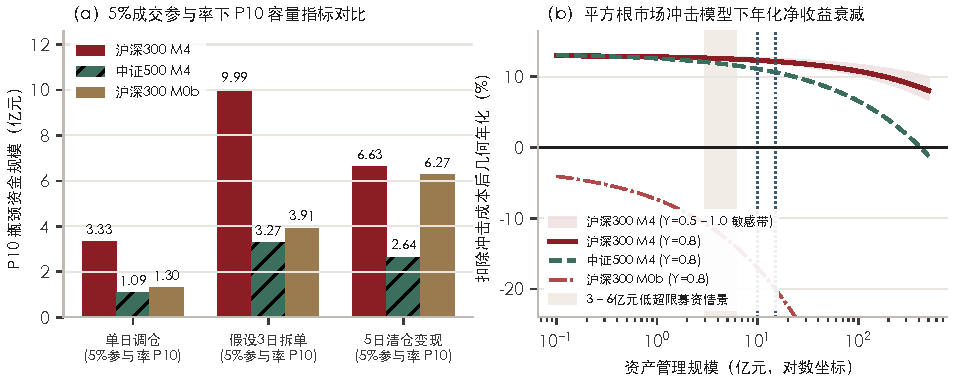
\includegraphics[width=\textwidth]{../figures/report_tex/fig10_capacity_impact.pdf}\\[-2pt]
{\color{Primary}\rule{\textwidth}{0.6pt}}\\[2pt]
\exhibitnote{资料来源：列祖列宗量化投研部测算。注：右图横轴为对数刻度资产管理规模（亿元），浅红色阴影带展示冲击系数 $Y \in [0.5, 1.0]$ 的参数敏感性区间。}
\end{minipage}
\vspace{5pt}

由于 P10 分位数指标在统计定义上仍允许 10\% 的尾部调仓期超出 5\% 参与率阈值，产品容量披露不宜简化为单一确定数字，而应按执行情景分层陈述：在 \textbf{3.00 亿元情景}下，沪深300 M4 单日集中调仓有 15/184 期（8.2\%）个别低流动性标的超过 5\% 参与率，假设拆分为 3 日均分执行或考察 5 日全部清仓则均为 \textbf{0 期超限}；在 \textbf{5.00 亿元情景}下，单日调仓有 \textbf{38/184 期（20.7\%）}超 5\% 参与率，假设拆为 3 日均分后仍有 \textbf{4/184 期（2.2\%）}超限，5 日清仓亦有 \textbf{1/185 期}轻微超限（最长需 \textbf{5.013 天}）；在 \textbf{10.00 亿元情景}下，假设 3 日均分拆单与 5 日清仓超限期数分别为 \textbf{18/184 期与 79/185 期}；在 \textbf{15.00 亿元情景}下则分别进一步升至 \textbf{38/184 期与 142/185 期}（最长需 15.040 天清仓）。此外必须指出执行口径差异：第三章主回测采用次日开盘集中撮合，而多日 TWAP/VWAP 拆单属于另一套独立交易执行情景，实盘若对超限尾部订单拉长执行窗口，还需额外承担拆单期间的价格漂移与信号衰减。综合评估，沪深300 M4 首期募资宜控制在 3 至 6 亿元并配合尾部限速拆单，10 亿元及 15 亿元规模仅作为需配套算法交易压测的远期扩张情景。

\subsection{5.4 雪球公开组合跟踪偏差回测与归档运行记录}

为开展公开模拟运行，团队在雪球平台建立了公开组合 \textbf{ZH3689205}（\url{https://www.xueqiu.com/P/ZH3689205}）。由于该平台限制单组合持仓上限为 30 只且仅接受整数百分比权重，无法直接录入 50 只各 2\% 的主策略目标清单，本研究将“50 股主回测”、“30 股历史映射回测”与“平台实际归档运行记录”三套口径严格分列（见图表 23 与图表 24）。

在 921 个交易日同一无前视回测引擎下，若将 M4 直接按当期排名硬截断取前 30 只（前 10 只各 4\%、第 11 至 30 只各 3\%）而不设独立缓冲，单次单边换手会由 50 股原组合的 2.74\% 反弹至 7.51\%；为 30 只分层方案专门匹配“前 45 名保留缓冲带”后，单次单边换手回落至 \textbf{3.15\%}，与 50 股原组合的日收益率相关系数达 \textbf{0.9676}，年化跟踪误差为 \textbf{3.75\%}。尽管 30 股前 45 缓冲方案在历史映射回测中因头部高分股权重集中而录得较高累计收益（+77.63\%），该数字仅用于评估平台制度约束下的跟踪误差，本研究对外主口径始终锁定为分散度更高的 50 股等权原组合（+56.58\%）。

\vspace{4pt}
\noindent\begin{minipage}{\textwidth}
\setlength{\parindent}{0pt}\setlength{\tabcolsep}{2.4pt}
\exhibitcap{图表 23：历史回测 50 股原组合、30 股历史映射与雪球公开组合运行记录分列对照表}
\fontsize{7.25pt}{9.9pt}\selectfont
\begin{tabularx}{\textwidth}{@{}l >{\raggedright\arraybackslash}X r r r r r r r@{}}
  \arrayrulecolor{Primary}\toprule[1.0pt]
  \rowcolor{TblHdr}
  \textbf{\sffamily 组合口径} & \textbf{\sffamily 持仓与缓冲规则} & \textbf{\sffamily 累计收益} & \textbf{\sffamily 几何年化} & \textbf{\sffamily 算术夏普} & \textbf{\sffamily 最大回撤} & \textbf{\sffamily 单次换手} & \textbf{\sffamily 年化TE} & \textbf{\sffamily 日相关} \\
  \rowcolor{TblHdr}
  {\fontsize{6.2}{7.6}\selectfont\textcolor{GrayNote}{（历史映射与实盘分列）}} &
  {\fontsize{6.2}{7.6}\selectfont\textcolor{GrayNote}{（权重合计100\%）}} &
  {\fontsize{6.2}{7.6}\selectfont\textcolor{GrayNote}{(\%)}} &
  {\fontsize{6.2}{7.6}\selectfont\textcolor{GrayNote}{(\%)}} &
  {\fontsize{6.2}{7.6}\selectfont\textcolor{GrayNote}{($r_f=0$)}} &
  {\fontsize{6.2}{7.6}\selectfont\textcolor{GrayNote}{(\%)}} &
  {\fontsize{6.2}{7.6}\selectfont\textcolor{GrayNote}{(\%/次)}} &
  {\fontsize{6.2}{7.6}\selectfont\textcolor{GrayNote}{(vs50,\%)}} &
  {\fontsize{6.2}{7.6}\selectfont\textcolor{GrayNote}{(vs50)}} \\
  \midrule[0.5pt]
    \multicolumn{9}{@{}l}{\textbf{\sffamily\textcolor{Primary}{A. 历史回测与30股映射回测口径（2023-01-09 至 2026-10-30，921个交易日，固定千1印花税情景）}}}\\[1pt]
    \textbf{\textcolor{Primary}{M4 主回测原组合}} & 50股各2\%（前75缓冲） & \textbf{\textcolor{Primary}{+56.58}} & \textbf{+13.05} & \textbf{0.905} & \textbf{-15.88} & \textbf{2.74} & 0.00 & 1.0000 \\
    M4 30股分层（含缓冲） & 前10×4\%+后20×3\%（前45缓冲） & +77.63 & +17.02 & 1.142 & -15.98 & 3.15 & 3.75 & 0.9676 \\
    M4 30股等权（含缓冲） & 30股各3.33\%（前45缓冲） & +80.07 & +17.46 & 1.170 & -15.14 & 2.67 & 3.60 & 0.9700 \\
    M4 30股截断（无缓冲） & 前10×4\%+后20×3\%（直取前30） & +71.53 & +15.91 & 1.068 & -16.03 & 7.51 & 3.57 & 0.9710 \\
    M0a 历史基线原组合 & 50股各2\%（无缓冲） & +41.56 & +9.98 & 0.673 & -17.02 & 5.83 & 0.00 & 1.0000 \\
    M0a 30股分层（建仓源） & 前10×4\%+后20×3\%（无缓冲） & +42.17 & +10.11 & 0.686 & -16.24 & 5.03 & 4.63 & 0.9580 \\
    \arrayrulecolor{RuleMuted}\midrule[0.4pt]
    \multicolumn{9}{@{}l}{\textbf{\sffamily\textcolor{Primary}{B. 雪球平台公开组合 ZH3689205 本地归档运行截面（平台实时撮合口径，读取人工核验记录）}}}\\[1pt]
    ZH3689205 归档运行截面 & 2026-11-18至11-23（30股分层） & -0.91 & — & — & — & — & — & — \\
  \arrayrulecolor{Primary}\bottomrule[1.0pt]
\end{tabularx}\\[3pt]
\exhibitnote{资料来源：面板 A 源自统一账户引擎下的 30 股映射回测账本；面板 B 源自本地归档截图人工核验记录（xueqiu\_screenshot\_verified.json）。}
\end{minipage}
\vspace{5pt}

\noindent\begin{minipage}{\textwidth}
\setlength{\parindent}{0pt}
\exhibitcap{图表 24：M4 50 股原组合与 30 股分层映射历史净值及单次换手率对比}
{\color{Primary}\rule{\textwidth}{0.8pt}}\\[2pt]
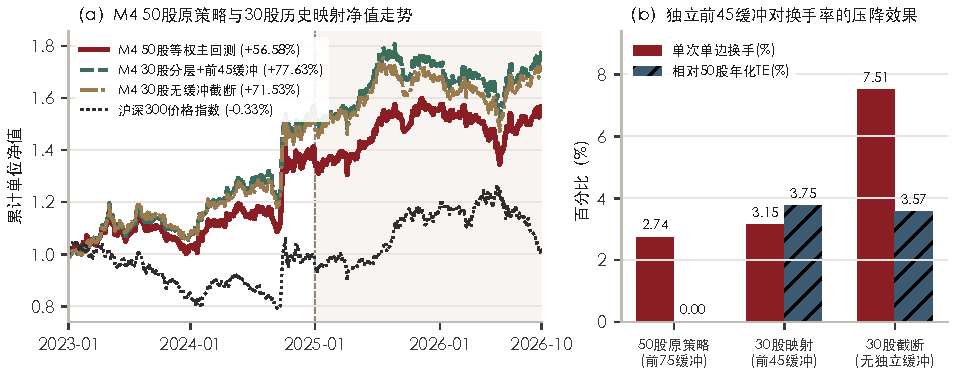
\includegraphics[width=\textwidth]{../figures/report_tex/fig11_xueqiu_tracking.pdf}\\[-2pt]
{\color{Primary}\rule{\textwidth}{0.6pt}}\\[2pt]
\exhibitnote{资料来源：列祖列宗量化投研部测算。}
\end{minipage}
\vspace{5pt}

在历史数据截止点（信号日 2026-10-29、执行日 2026-10-30），M4 完整 50 只历史末期目标持仓中综合得分居前五位的标的依次为 华夏银行（600015.SH，银行）、中国铁建（601186.SH，建筑装饰）、光大银行（601818.SH，银行）、中国中铁（601390.SH，建筑装饰）、上汽集团（600104.SH，汽车）。图表 25 列出该截止日前最近 8 个常规调仓周期的真实换手与标的进出对账：8 期中有 4 期实现零标的更替（仅因价格漂移产生 0.62\% 至 0.94\% 的权重再平衡换手），其余 4 期每次仅更替 1 至 2 只股票，近 8 期平均单次单边换手为 \textbf{2.13\%}。

\vspace{4pt}
\noindent\begin{minipage}{\textwidth}
\setlength{\parindent}{0pt}\setlength{\tabcolsep}{3.8pt}
\exhibitcap{图表 25：主交付策略 M4 历史末期近 8 期（2026.09--2026.10）调仓换手与标的更替明细表}
\fontsize{7.7pt}{10.4pt}\selectfont
\begin{tabularx}{\textwidth}{@{}l l r c X X@{}}
  \arrayrulecolor{Primary}\toprule[1.0pt]
  \rowcolor{TblHdr}
  \textbf{\sffamily 调仓执行日} & \textbf{\sffamily 信号生成日} & \textbf{\sffamily 单边换手(\%)} & \textbf{\sffamily 买/卖只数} & \textbf{\sffamily 新调入标的} & \textbf{\sffamily 全卖出标的} \\
  \midrule[0.5pt]
    2026-09-03 & 2026-09-02 & 3.05 & 1 / 1 & 中联重科(000157.SZ) & 中国中冶(601618.SH) \\
    2026-09-10 & 2026-09-09 & 0.76 & 0 / 0 & 无（全保留） & 无（全保留） \\
    2026-09-17 & 2026-09-16 & 0.94 & 0 / 0 & 无（全保留） & 无（全保留） \\
    2026-09-24 & 2026-09-23 & 0.62 & 0 / 0 & 无（全保留） & 无（全保留） \\
    2026-10-09 & 2026-10-08 & 0.91 & 0 / 0 & 无（全保留） & 无（全保留） \\
    2026-10-16 & 2026-10-15 & 3.09 & 1 / 1 & 新华保险(601336.SH) & 京沪高铁(601816.SH) \\
    2026-10-23 & 2026-10-22 & 2.84 & 1 / 1 & 大华股份(002236.SZ) & 中国石化(600028.SH) \\
    2026-10-30 & 2026-10-29 & 4.83 & 2 / 2 & TCL科技(000100.SZ)、中国电建(601669.SH) & 格力电器(000651.SZ)、交通银行(601328.SH) \\
  \arrayrulecolor{Primary}\bottomrule[1.0pt]
\end{tabularx}\\[3pt]
\exhibitnote{资料来源：实际开盘持仓与调仓账本导出的近8期调仓审计表。}
\end{minipage}
\vspace{5pt}

关于雪球公开组合 \textbf{ZH3689205} 的平台实际运行记录，依据本地归档截图人工核验记录（见图表 26）：该组合于 \textbf{2026-11-18 18:30:50} 按前期历史基线 M0a 的 30 股分层映射（前 10 只各 4\% 加后 20 只各 3\%，共 30 只标的、目标权重合计 100\%）完成首次建仓；截至本地最新归档概览截面 \textbf{2026-11-23}，组合单位净值为 \textbf{0.9909}，建仓以来累计收益为 \textbf{-0.91\%}，同期沪深300基准变动为 \textbf{-0.64\%}（仅数个交易日的极短运行窗口不具统计显著性，作为公开模拟盘真实运行留痕）。此外，研究团队于 2026-11-25 基于实时成分行情生成了向 M4（30 股分层、前 45 名保留缓冲）过渡的拟议调仓指令单；经逐只按股票代码核对确认，2026-11-18 建仓截图中的 30 只股票及 4\%/3\% 目标权重与该操作单所采用的起始持仓完全一致，据此测算的\textbf{拟议切换单边换手为 16.00\%}（保留 26 只、调出 4 只、新调入 4 只）。本地归档凭证目前支持平台运行披露至 2026-11-23，M4 规则在雪球平台上的正式生效日以平台调仓成交回执为准。

\vspace{4pt}
\noindent\begin{minipage}{\textwidth}
\setlength{\parindent}{0pt}
\exhibitcap{图表 26：雪球公开模拟组合 ZH3689205 本地归档运行概览（截至 2026-11-23）与首次 30 股建仓截图凭证}
{\color{Primary}\rule{\textwidth}{0.8pt}}\\[3pt]
\begin{tabularx}{\textwidth}{@{}>{\centering\arraybackslash}X >{\centering\arraybackslash}X@{}}
  \fcolorbox{RuleMuted}{white}{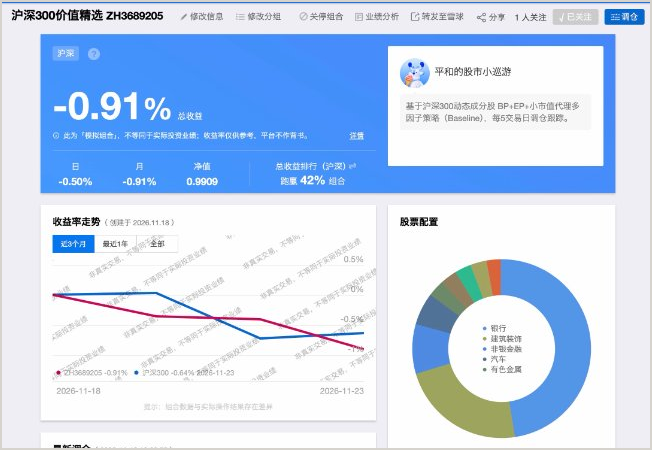
\includegraphics[width=0.47\textwidth,height=4.9cm,keepaspectratio]{../xueqiu/screenshots/xueqiu_ZH3689205_overview_20261123.png}} &
  \fcolorbox{RuleMuted}{white}{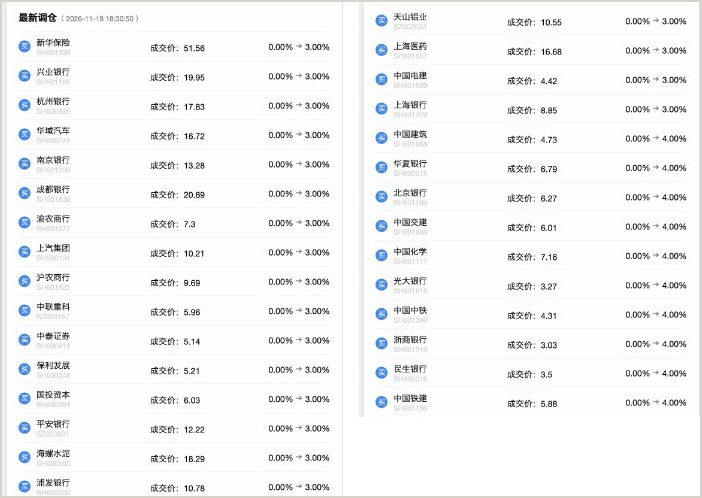
\includegraphics[width=0.47\textwidth,height=4.9cm,keepaspectratio]{../xueqiu/screenshots/xueqiu_ZH3689205_rebalance_20261118.png}} \\[2pt]
  {\fontsize{7.3pt}{9.5pt}\selectfont\textcolor{SubInk}{（a）2026-11-23 组合净值与收益概览归档截图}} &
  {\fontsize{7.3pt}{9.5pt}\selectfont\textcolor{SubInk}{（b）2026-11-18 18:30:50 首次 30 股分层建仓明细截图}}
\end{tabularx}\\[2pt]
{\color{Primary}\rule{\textwidth}{0.6pt}}\\[2pt]
\exhibitnote{资料来源：雪球平台公开组合页面（\url{https://www.xueqiu.com/P/ZH3689205}）本地归档截图，相关数值经人工逐项核验录入元数据文件统一引用。}
\end{minipage}
\vspace{4pt}

% =========================================================================
% 六、关键方法学讨论、模型局限与风险提示
% =========================================================================
\section{六、关键方法学讨论、模型局限与风险提示}

\subsection{6.1 样本期切分边界、分红口径差异与选型权衡复盘}

为保障研究结论经得起投委会与学术同行审视，本节对三项关键方法学边界作集中说明：

第一，\textbf{历史留后区间的属性界定。}本研究的因子方向、Alpha101 重筛入选名单与多重检验阈值均严格锁定在 2019–2022 年训练期内生成；但在从早期数据底座升级至 Tushare 双股票池、诊断 Alpha015 覆盖率约束以及比较 M1 至 M5 控制变量序列的过程中，2025 年 1 月至 2026 年 10 月的回测表现已进入团队讨论视野并辅助了跨池稳健性判断。因此，该时间段在方法学属性上属于“已参与方案讨论的历史留后区间”，真正的严格前瞻样本外表现须依托模型规则冻结后自 2026 年 11 月起持续累积的新行情与平台调仓回执加以检验。

第二，\textbf{组合后复权分红再投资与价格指数基准的股息口径差异。}本报告中策略账户净值基于个股后复权价格计算，隐含了成分股现金分红在除息日按复权比例再投资的收益；而随包历史基准数据仅包含沪深300价格指数（000300.SH）与中证500价格指数（000905.SH），价格指数在成分股派息除权时自然回落而不计入现金股息。按价格指数口径，沪深300 M4 全期累计净收益（+56.58\%）与沪深300价格指数（-0.33\%）的累计收益差为 +56.90 个百分点；若按沪深300近年约 2.5\% 至 3.0\% 的年化股息率做粗略情景估算，近 3.65 年样本期内现金分红复利约贡献 10 至 12 个百分点的基准收益差。需要强调，这一扣减区间仅为量级层面的情景参考，由于价值低波高股息组合自身的股息率亦高于宽基均值，精确度量含分红基准超额收益以及重算方案 B、方案 C 的超额业绩报酬，有赖于后续接入同起点的沪深300全收益指数（H00300.CSI）。

第三，\textbf{选定 M4 的证据边界复盘。}本报告并不宣称 M4 在单一股票池的每一项指标或每一个子区间均占优：在沪深300池内，M4 的历史留后区间收益低于 M1、最大回撤略深于 M1，且全期收益与夏普低于五因子 M5。选定 M4 的依据严格停留在双池对照与归因证据能够支持的位置：其一，减少一个由 EP/BP 直接派生的比率因子，避免了该比率在中证500池产生的显著负向暴露拖累（-2.90 个百分点/年）；其二，完全同一套四因子等权与缓冲参数在沪深300与中证500上分别取得 +56.58\% 与 +57.73\% 的扣费累计净收益及 0.905 与 0.816 的算术夏普，展现出较好的跨市值层级一致性。

\subsection{6.2 数据与执行假设局限及后续改进方向}

当前研究与工程实现仍存在四项客观局限，构成下一阶段迭代的具体方向：（1）\textbf{财务质量因子的时点数据条件}，现有数据底座虽对日频估值施加了 90 天龄期上限，但尚未接入带精确首次披露与更正时间戳的季度财务报表 Point-in-Time 数据库，因此暂未纳入真实现金流质量、毛利率变动或标准化预期外盈利（SUE）等基本面成长因子；（2）\textbf{撮合粒度与大单算法执行差距}，回测采用次日开盘价叠加固定千 1 滑点的集中成交假设，尚未利用日内分钟线或逐笔委托簿还原开盘集合竞价可成交量上限，对于 5 亿元以上规模出现的参与率超限调仓期，需进一步构建嵌入多日拆单路径的回测器；（3）\textbf{组合构建尚采用启发式等权与排名缓冲}，在面向机构定制专户落地单行业 $\le 35\%$ 上限及个股跟踪误差预算时，宜升级为显式包含线性行业约束、个股流动性权重上限与换手率线性惩罚项的均值—方差或二次规划（QP）组合优化器；（4）\textbf{股息再投资摩擦}，后复权价格隐含税前分红即时再投资，实盘私募基金需按持股期限适用差异化股息红利个人所得税代扣规则（或机构税盾规则）并承担现金分红到账滞后。

\subsection{6.3 风险提示与合规声明}

\begin{enumerate}[leftmargin=2.2em, itemsep=2pt, topsep=3pt]
  \item \textbf{模型失效与市场风格切换风险：}本策略基于历史统计规律构建，核心收益依赖大盘价值估值修复与低波动、低换手防御因子的长期风险溢价。当宏观流动性宽松或产业周期驱动市场进入高估值成长股、高换手主题股单边领涨阶段时，组合可能出现持续数月跑输宽基基准的相对回撤。
  \item \textbf{金融行业持仓集中度风险：}在无行业硬上限约束的基准设定下，沪深300 M4 对申万一级银行及非银金融板块的全期平均持仓达 42.4\%、期末达 50.0\%。宏观利率环境、银行业净息差政策或金融监管政策变动可能对组合净值造成集中波动冲击。
  \item \textbf{流动性冲击与容量超限风险：}历史压测表明，在 5.00 亿元及以上资产规模下，部分调仓期存在单日成交参与率超过 5\% 的低流动性成分股；若遇极端市场恐慌导致全市场成交萎缩或连续跌停，实际变现滑点与清仓周期可能超出历史正常行情估算值。
  \item \textbf{历史回测与模拟表现局限声明：}本报告中的历史回测净值、产品费后历史模拟净值及雪球公开模拟盘记录仅供《量化交易技术理论与实践》课程学术评审与模拟投委会讨论使用，不代表真实基金产品过往业绩，亦不构成对任何证券或私募产品的投资建议与收益承诺。
\end{enumerate}

\newpage

% =========================================================================
% 参考文献与附录 A
% =========================================================================
\section{参考文献}

{\setlength{\parindent}{0pt}\fontsize{10.5pt}{15.5pt}\selectfont
\begin{enumerate}[leftmargin=2.1em, itemsep=3.5pt, topsep=0pt, label={[\arabic*]}]
  \item Ang, A., Hodrick, R. J., Xing, Y., \& Zhang, X. (2006). The cross-section of volatility and expected returns. \textit{The Journal of Finance}, 61(1), 259--299.
  \item Almgren, R., Thum, C., Hauptmann, E., \& Li, H. (2005). Direct estimation of equity market impact. \textit{Risk}, 18(7), 58--62.
  \item Datar, V. T., Naik, N. Y., \& Radcliffe, R. (1998). Liquidity and stock returns: An alternative test. \textit{Journal of Financial Markets}, 1(2), 203--219.
  \item Fama, E. F., \& French, K. R. (1993). Common risk factors in the returns on stocks and bonds. \textit{Journal of Financial Economics}, 33(1), 3--56.
  \item Fama, E. F., \& MacBeth, J. D. (1973). Risk, return, and equilibrium: Empirical tests. \textit{Journal of Political Economy}, 81(3), 607--636.
  \item Frazzini, A., \& Pedersen, L. H. (2014). Betting against beta. \textit{Journal of Financial Economics}, 111(1), 1--25.
  \item Grinold, R. C., \& Kahn, R. N. (2000). \textit{Active Portfolio Management: A Quantitative Approach for Producing Superior Returns and Controlling Risk} (2nd ed.). McGraw-Hill.
  \item Holm, S. (1979). A simple sequentially rejective multiple test procedure. \textit{Scandinavian Journal of Statistics}, 6(2), 65--70.
  \item Kakushadze, Z. (2016). 101 Formulaic Alphas. \textit{Wilmott}, 2016(84), 72--81.
  \item Newey, W. K., \& West, K. D. (1987). A simple, positive semi-definite, heteroskedasticity and autocorrelation consistent covariance matrix. \textit{Econometrica}, 55(3), 703--708.
  \item 中华人民共和国财政部、国家税务总局. 关于减半征收证券交易印花税的公告（财政部 税务总局公告 2023 年第 39 号，自 2023 年 8 月 28 日起实施）[EB/OL]. 2023-08-27.
\end{enumerate}\par}

\vspace{10pt}

\section{附录 A：可复现工程架构与报告术语—代码字段映射表}

遵循课程书面研究报告正文不插入程序代码片段的规范，本研究全部数据处理、因子重筛、账户回测、容量费率测算及本报告的动态矢量图与 XeLaTeX 编译脚本均已托管至开源仓库（\url{https://github.com/z2823253773-p/csi300-quant-strategy}）。为便于审阅人核对仓库源码与结果表，图表 27 汇总了四阶段工程模块、底层数据来源属性以及报告正文规范金融术语与仓库代码字段的一一对应关系。

\vspace{4pt}
\noindent\begin{minipage}{\textwidth}
\setlength{\parindent}{0pt}\setlength{\tabcolsep}{3.6pt}
\exhibitcap{图表 27：全链路可复现工程模块、数据来源属性与报告术语—代码字段映射表}
\fontsize{7.5pt}{10.2pt}\selectfont
\begin{tabularx}{\textwidth}{@{}l l l X@{}}
  \arrayrulecolor{Primary}\toprule[1.0pt]
  \rowcolor{TblHdr}
  \textbf{\sffamily 工程阶段 / 报告术语} & \textbf{\sffamily 仓库目录或核心文件} & \textbf{\sffamily 代码字段 / 变量标识} & \textbf{\sffamily 数据来源属性与可复现校验说明} \\
  \midrule[0.5pt]
  阶段1：双池数据治理 & \texttt{member1\_data/} & \texttt{fetch\_tushare.py} & 个股行情/估值/复权/ST取自Tushare；成分/行业/指数取自 \texttt{seed/} \\
  阶段2：因子重筛与信号 & \texttt{member2\_signals/} & \texttt{run\_pool.py, check\_015.py} & 生成 101 重筛表、M0a--M5 目标权重与 Alpha015 退出审计 CSV \\
  阶段3：无前视回测归因 & \texttt{member3\_backtest/} & \texttt{run\_backtest\_v3.py} & 生成 63 组日净值、绩效主表、行业暴露与 7 因子 FM 归因 CSV \\
  阶段4：产品与动态排版 & \texttt{member4\_product/} & \texttt{build\_report\_tex\_v3.py} & 动态读取上游 CSV/JSON 编译 11 张矢量图与本 PDF 技术报告 \\
  \arrayrulecolor{RuleMuted}\midrule[0.35pt]
  干净共同池 / 含015池 & \texttt{metrics\_v3.csv} & \texttt{hs300\_clean / hs300\_full} & 区分解除 Alpha015 覆盖约束主消融池与原总交集专题对照池 \\
  固定千1 / 历史减半税率 & \texttt{metrics\_v3.csv} & \texttt{net\_10bp / net\_histtax} & 分别对应全期固定卖出10bp印花税与2023-08-28起减半至5bp情景 \\
  历史留后区间 & \texttt{metrics\_v3.csv} & \texttt{stage = seen} & 对应 2025-01-02 至 2026-10-30（已参与方案讨论，非盲测集） \\
  原始有效交易观测掩码 & \texttt{operators.py} & \texttt{valid, open\_quote\_observed} & 正常交易、非停牌、报价齐全且成交量 $>0$；滚动计算前置掩码 \\
  对数流通市值与小市值 & \texttt{models.py} & \texttt{ln\_float\_mv\_proxy, small} & 由日成交额除以换手率构造，覆盖率 100\% \\
  成交额平滑改造012 & \texttt{factor\_ic\_v3.csv} & \texttt{new012\_amt\_ema10} & 相对日收益乘以成交额变化负符号再经 10 日 EMA 平滑 \\
  隐含账面盈利率代理 & \texttt{decomp\_v3.csv} & \texttt{eb\_proxy} & 由 \texttt{ep / bp} 直接相除构造的比率因子，仅用于 M5 对照与归因 \\
  雪球截图人工核验记录 & \texttt{member4\_product/xueqiu/} & \texttt{xueqiu\_screenshot\_verified.json} & 记录人工核验的 2026-11-18 建仓与 11-23 概览截图指标及路径 \\
  \arrayrulecolor{Primary}\bottomrule[1.0pt]
\end{tabularx}\\[3pt]
\exhibitnote{资料来源：列祖列宗量化投研部整理。注：回测、归因、容量与费率数据均由脚本直接读取 CSV/JSON 自动填入；雪球平台页面快照指标因无公开导出接口，由团队核对归档截图后录入上述结构化核验记录供正文与表格共同引用。}
\end{minipage}

\end{document}
